\chapter{Assesment of Transcriptional Induction, Expression, and Subcellular Localisation of Human and Bovine IFITs in the Context of RSV} \label{Assesment of Transcriptional Induction, Expression, and Subcellular Localisation of Human IFITs in the Context of RSV}
\section{Introduction and Aims} \label{Introduction and Aims}
\textbf{Half page intro:}
Ifit gene regulation (promoters and such) \newline
Ifit paths of induction \newline
interferons \newline
Lps tlr4 \newline
Poly IC \newline
Ifit induction by other viruses and inducers \newline


\textbf{Half page aims:}
We hypothesised both human and bovine IFITs to be induced by human and bovine RSV infection. We aimed to systematically test this by initially confirming that our model cell lines are capable of IFIT induction following the treatment of known innate immune system activators such as interferons, LPS, and poly I:C. These would also allow us to assess the  We would then assess the IFIT induction during human and bovine RSV infection using a range of viral concentrations and end assay time points. Lastly, we would validate this data in more physiologically relevant cell lines as well as using omics approaches.

\section{Results} \label{Results}

\subsection{Transcriptional Changes of Human and Bovine \textit{IFITs}} \label{Transcriptional Changes of Human and Bovine \textit{IFITs}}
To unravel the impact of cellular stimulation with activators of the innate immune response and either human RSV or bovine RSV, on the expression of human and bovine \textit{IFIT} genes, quantitative real-time reverse transcription PCR (qPCR) analysis was executed in accordance with the methodology outlined in Section \ref{Quantitative Real Time/Reverse Transcription PCR}. Briefly, cells were cultivated in 12-well plates and subsequently subjected to the respective stimulants. At the endpoint of the experiments, the RNA was extracted, followed by cDNA synthesis and the transcript quantification by qPCR. All transcript levels were standardized to either human or bovine \textit{GAPDH} expression, employing either the 
\(\Delta\)\(\Delta\)Ct method or, in the case of bovine \textit{IFITs}, initial copy number assessment. Subsequently, all values were normalized against mock-treated samples, enabling data aggregation and inter-experimental induction value comparison. The statistical analysis was conducted as outlined in Section \ref{Statistical Analysis}. Notably, the choice of the appropriate statistical test hinged on the normality of data distribution and equality of variance, aspects which will be underscored in the ensuing text.




\subsubsection{Bovine \textit{IFIT} qPCR Primer Validation} \label{Bovine IFIT qPCR Primer Validation}

Due to the initial lack of commercially available primers for the detection of bovine \textit{IFIT} transcripts at the outset of the project, I devised a panel comprising three primer sets (PS) for each bovine \textit{IFIT} gene. Detailed information about this process is outlined in Section \ref{Primer Design and Assay Setup}. In a nutshell, I inputted the coding sequences into the PrimerQuest software (Integrated DNA Technologies) to identify the most suitable oligonucleotides. To evaluate the amplification efficiencies of each primer set, I employed \textit{IFIT} DNA clones from a bovine ISG library as standards (accessible through a collaboration with CVR Glasgow). The outcomes are depicted in Figure \ref{Validation of custom-made bIFIT qPCR primers}. The graph demonstrates that primer sets 1 exhibited the most favourable amplification efficiencies. All primer sets, except for \textit{bIFIT3}, yielded nearly impeccable amplification efficiencies of around 100\%. Consequently, they were chosen for subsequent experiments. While \textit{bIFIT3} primer sets demonstrated similar outcomes in terms of standard curve slopes and amplification efficiencies, PS1 consistently outperformed the others in repeated testing rounds (data not presented). As a result, it was singled out for further experimentation.

\begin{figure}
    \centering
    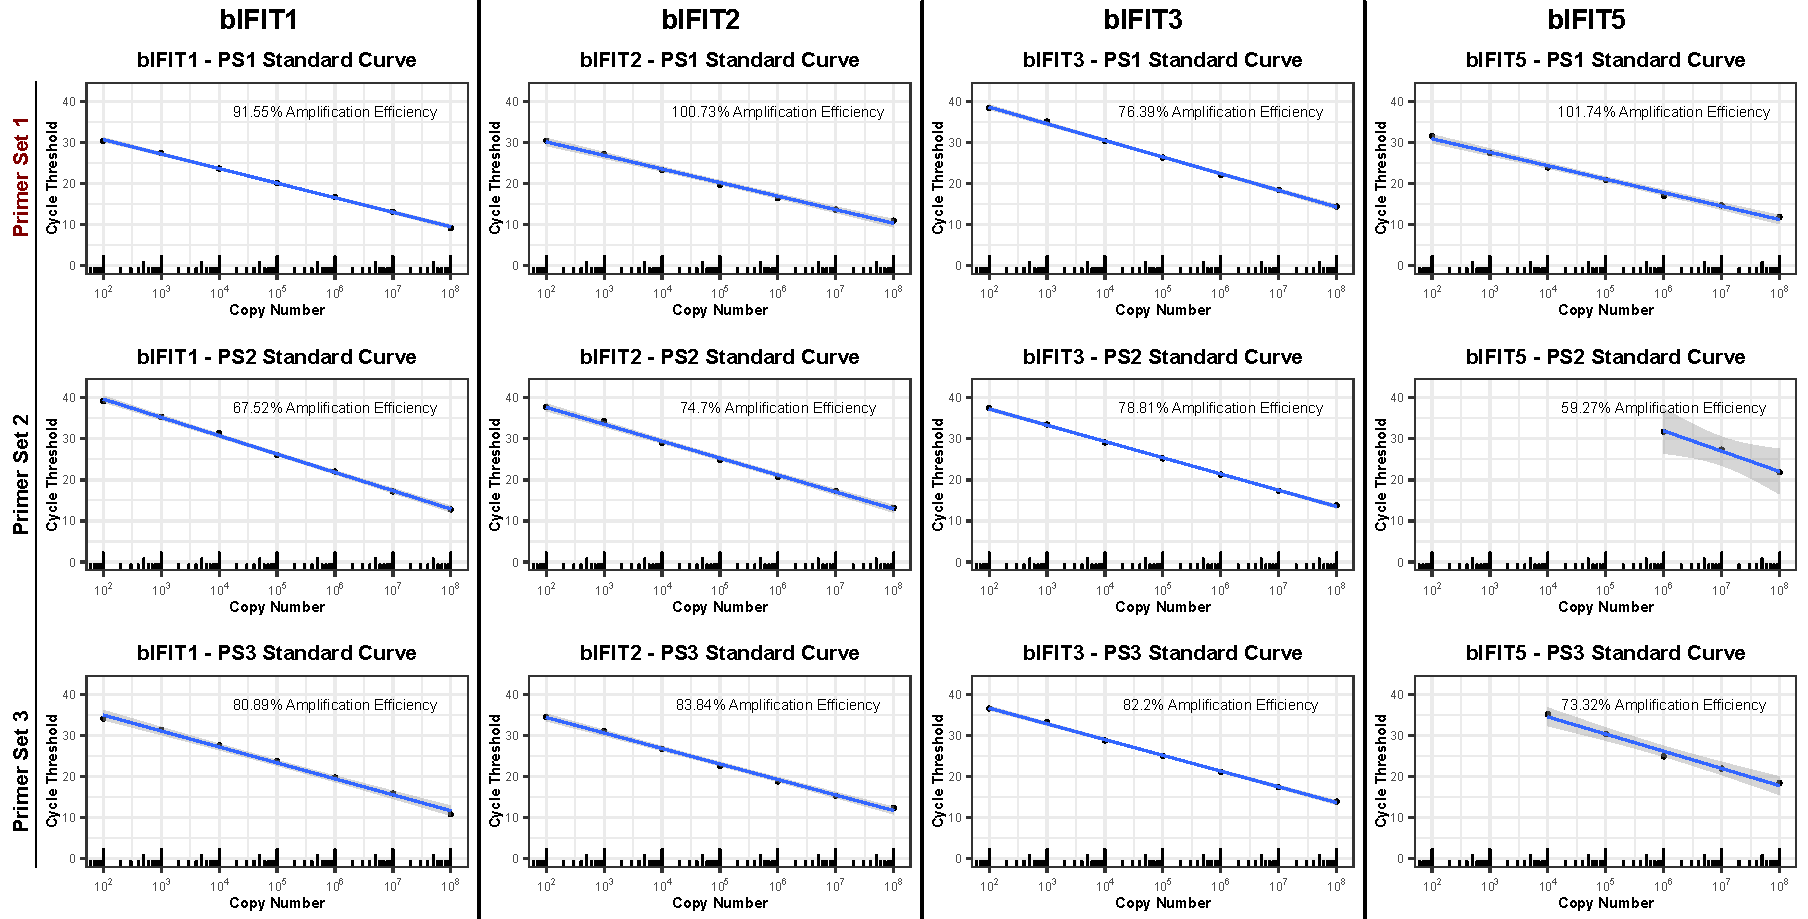
\includegraphics[width=1\linewidth]{07. Chapter 2/Figs/01. Technologies/02. primer validation.pdf}
    \caption[Validation of Custom-Made \textit{bIFIT} qPCR Primers.]{\textbf{Validation of Custom-Made \textit{bIFIT} qPCR Primers.} The custom-designed primers were evaluated by creating a serial dilution of bovine \textit{IFIT}-containing plasmids, provided by the CVR Glasgow. The resulting standard curves are shown here. Primer set (PS) 1 (a), 2 (b), and 3 (c) are depicted for bovine \textit{IFIT1} (1.), \textit{IFIT2} (2.), \textit{IFIT3} (3.), and \textit{IFIT5} (4.), along with their calculated amplification efficiencies.}
    \label{Validation of custom-made bIFIT qPCR primers}
\end{figure}

The PSs behaviour was monitored throughout the project, as fresh standard curves were created per experiment. Figure \ref{The Performance of Custom-Made Primer-Sets Over Time} shows that the average data is consistent with what was observed in initial testing (Figure \ref{Validation of custom-made bIFIT qPCR primers}), however, there were per experiment deviations in slope angles for each of the selected primer pairs. The underlying amplification efficiencies stayed consistent, as is highlighted by the averaged efficiencies displayed. The initial \textit{bIFIT3} PSs differential amplification slopes compared to the other \textit{bIFIT} PSs, as well as the variable nature of PSs performance throughout the project prohibits the usage of \(\Delta\)\(\Delta\)Ct methodologies for transcript quantification as the increase in cycle threshold would not be proportional to the decrease of transcript abundance between the \textit{bIFITs}, and thus a different methodology had to be adopted. This is described in detail in Section \ref{Data Processing}. In short, the copy numbers were deducted from standard curves and factorised by the relative abundance of bovine \textit{GAPDH}. This ensured the slope-independent establishment of relative expression values, mirroring and complementing data from \(\Delta\)\(\Delta\)Ct methodologies.

\begin{figure}
    \centering
    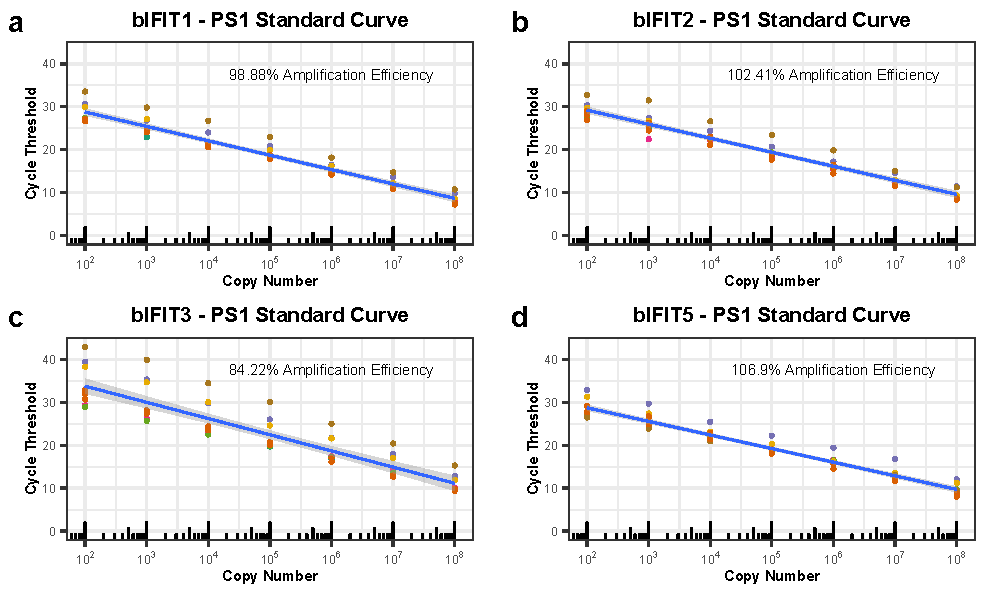
\includegraphics[width=1\linewidth]{07. Chapter 2/Figs/01. Technologies/03. standard curves behaviour.pdf}
    \caption[The Performance of Custom-Made Primer-Sets Over Time.]{\textbf{The Performance of Custom-Made Primer-Sets Over Time.} During the experiments with custom-made \textit{bIFIT} qPCR primers, standard curves had to be always constructed. Here, the underlying average amplification efficiencies and standard curves, along with the individual data, from all the experiments and coloured by the experiment are displayed.}
    \label{The Performance of Custom-Made Primer-Sets Over Time}
\end{figure}


















\subsubsection{Responses of to Known Activators of Innate Immune Response} \label{Responses to Known Activators of Innate Immune Response}
In order to establish the expression competency of \textit{IFIT} of the cell lines used, along with elucidating how different innate immune pathways contribute to the overall expression profile, I treated the cells with differing activators of the innate immune response. As described in Section \ref{Routes of IFIT Expression Activation}, and depicted in Figure \ref{Pathways Inducing ISG mRNA Production.},  interferon-stimulated genes (ISGs) can have their induction activated either via the interferon receptor signalling, intracellular foreign nucleic acid detection or via extracellular PAMP sensing. The latter, in the context of RSV, includes stimulation of TLR4 with either LPS or RSV particles. After surveying the literature I ended up using 1,000 international units (IU) per mL or the equivalent amount of 5 ng/mL for human and bovine interferon alpha respectively (\cite{Terenzi2006DistinctISG56}; \cite{Santhakumar2018ChickenViruses}). For interferon-gamma stimulation, which stimulates predominantly immune cells \textit{in vivo} concentrations of 500, 1,000 and 2,000 IU/mL were used. LPS was used in the concentration range of 0.5-10 ng/mL for the stimulation of bovine cells and in concentrations of 5 ng/mL and 2 \(\mu\)g/mL for the stimulation of human cells (\cite{Mears2019Ifit1Cells}; \cite{Zhang2019GrouperResponse}). To stimulate intracellular foreign nucleic acid recognition 2 \(\mu\)g of poly I:C were transfected into A549 cells and incubated for 24 hours (\cite{Mears2019Ifit1Cells}; \cite{Palchetti2015TransfectedCells}).

\begin{figure}
    \centering
    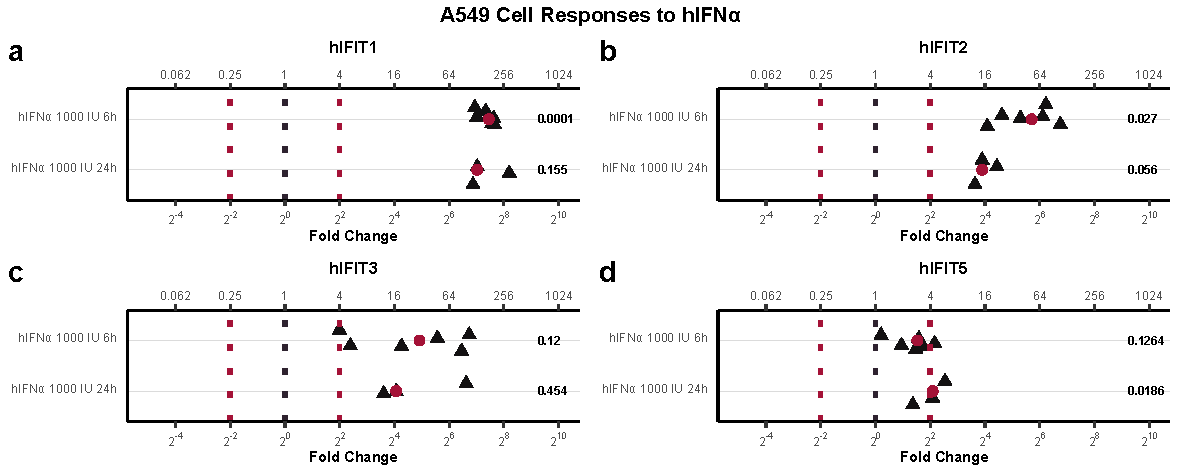
\includegraphics[width=1\linewidth]{06. Chapter 1/Figs/01. Induction/01. a549_treat_ifna.pdf}
    \caption[qPCR Analysis of A549 \textit{hIFIT} Response to hIFN\(\alpha\).]{\textbf{qPCR Analysis of A549 \textit{hIFIT} to hIFN\(\alpha\).} The relative abundance of (a) \textit{hIFIT1}, (b) \textit{hIFIT2}, (c) \textit{hIFIT3}, and (d) \textit{hIFIT5} genes, extracted from the A549 cell line, with response to human interferon alpha (IFN\(\alpha\)) at a concentration of 1000 IU per mL for a treatment duration of 6 or 24 hours. The shown values are relative to standardised mock values. The red circles signify median values. The black dotted line indicates mock expression, while the red dotted lines indicate biologically significant levels of induction. Numeric values signify the p-values compared to mock.}
    \label{A549 Response to hIFNa}
\end{figure}

We observe that after the stimulation of the A549 cell line with 1,000 IU/mL of hIFN\(\alpha\) for either 6 or 24 hours human \textit{IFIT1}, \textit{IFIT2}, and \textit{IFIT3} were induced drastically, especially \textit{IFIT1}, which was induced around 200-fold (Figure \ref{A549 Response to hIFNa}). The relative induction levels were identical between \textit{IFIT2} and \textit{IFIT3}. For all of these 3 genes, we can observe a decreased expression with longer incubation of IFN\(\alpha\), i.e. approximately half of the induction levels caused by 6-hour long incubation. Human \textit{IFIT5} shows minimal induction compared to the other \textit{IFITs} (3 and 4-fold for 6 and 24-hour long incubation respectively), which hovers around the mark of what is considered biologically significant induction, especially for ISGs, which are supposed not to be highly basally expressed. We can also observe a reverse trend of the time dependency of hIFN\(\alpha\)-induced expression. This suggests differential induction sensitivities between \textit{hIFIT1} (highly induced), \textit{hIFIT2} and \textit{hIFIT3} (medium induced) and \textit{hIFIT5} (low induced). All \textit{hIFIT} values had normal distributions and unequal variance other than \textit{hIFIT5}, which had normal distribution and normal variance.

\begin{figure}
    \centering
    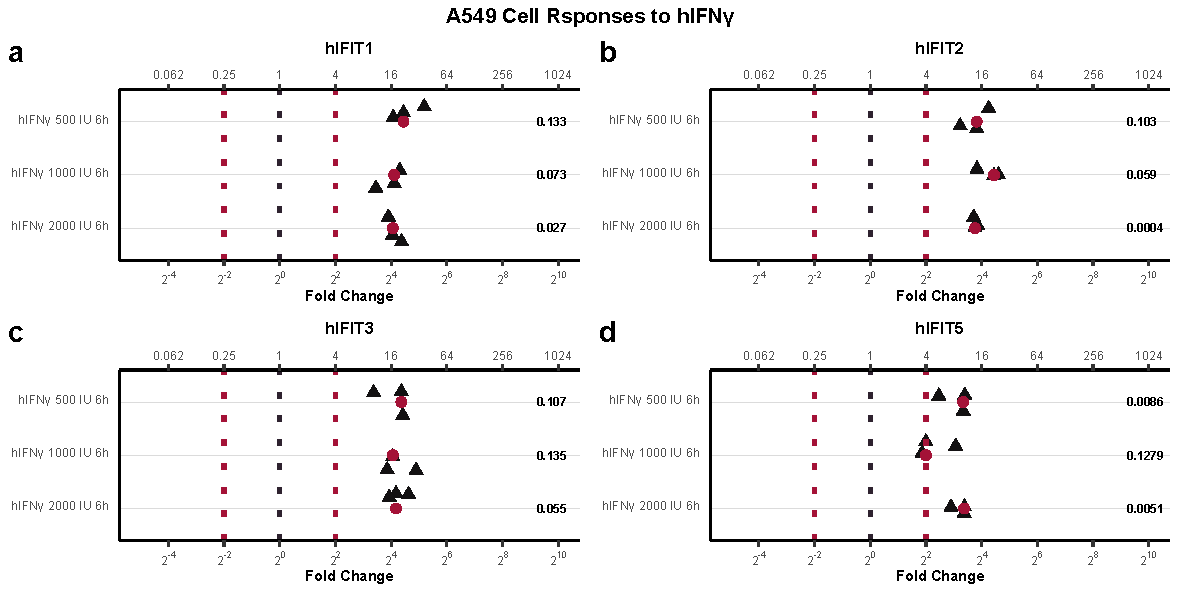
\includegraphics[width=1\linewidth]{06. Chapter 1/Figs/01. Induction/02. a549_treat_ifng.pdf}
    \caption[qPCR Analysis of A549 \textit{hIFIT} Response to hIFN\(\gamma\).]{\textbf{qPCR Analysis of A549 \textit{hIFIT} Response to hIFN\(\gamma\).} The relative abundance of (a) \textit{hIFIT1}, (b) \textit{hIFIT2}, (c) \textit{hIFIT3}, and (d) \textit{hIFIT5} genes, extracted from the A549 cell line, with response to human interferon-gamma (IFN\(\gamma\)) at concentrations of 500, 1000, and 2000 IU per mL for a treatment duration of 6 hours. The shown values are relative to standardised mock values. The red circles signify median values. The black dotted line indicates mock expression, while the red dotted lines indicate biologically significant levels of induction. Numeric values signify the p-values compared to mock.}
    \label{A549 Response to hIFNg}
\end{figure}

The response of human \textit{IFIT} genes to human IFN gamma can be seen in Figure \ref{A549 Response to hIFNg}. We can observe all \textit{IFITs} other than \textit{hIFIT5} responding equally to all concentrations tested i.e. 500, 1,000 and 2,000 IU/mL. Their response was concentration independent of a magnitude of around 15-fold. \textit{hIFIT5} response to very low concentration and very high concentrations was around 10-fold, while its transcript abundance increased only 4 times when treated with 1,000 IU/mL concentration. This suggests that the interferon-gamma component of the human \textit{IFIT} response is relatively equal for all of the \textit{IFIT} genes. This data, along with the data from hIFN\(\alpha\) induction also confirms that the A549 cell line is \textit{hIFIT} induction capable, which is great. All \textit{hIFIT} values had normal distributions and unequal variance other than \textit{hIFIT5}, which had normal distribution and normal variance.

\begin{figure}
    \centering
    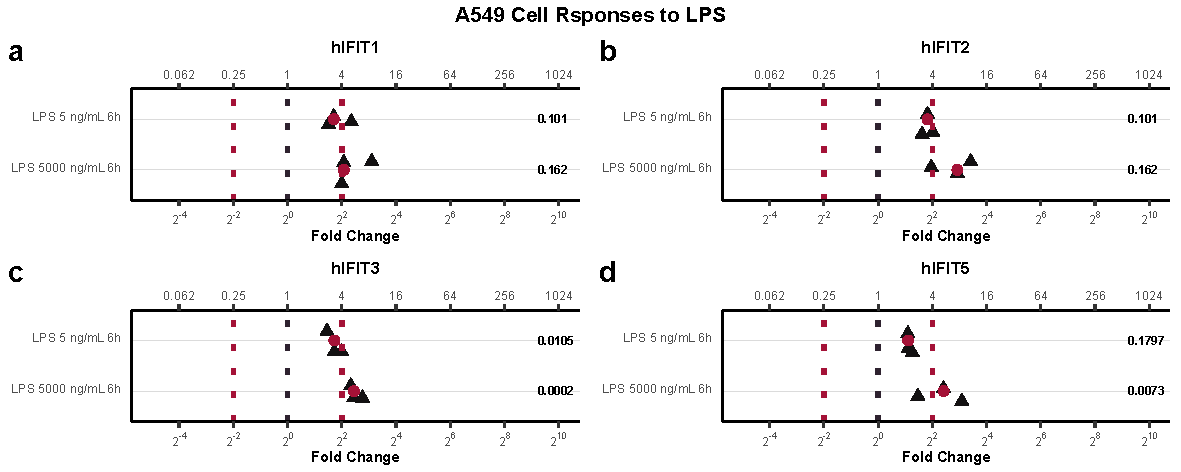
\includegraphics[width=1\linewidth]{06. Chapter 1/Figs/01. Induction/03. a549_treat_lps.pdf}
    \caption[qPCR Analysis of A549 \textit{hIFIT} Response to LPS.]{\textbf{qPCR Analysis of A549 \textit{hIFIT} Response to LPS.} The relative abundance of (a) \textit{hIFIT1}, (b) \textit{hIFIT2}, (c) \textit{hIFIT3}, and (d) \textit{hIFIT5} genes, extracted from the A549 cell line, with response to lipopolysaccharide (LPS) at concentrations of 5 and 5000 ng/mL for a treatment duration of 6 hours. The shown values are relative to standardised mock values. The red circles signify median values. The black dotted line indicates mock expression, while the red dotted lines indicate biologically significant levels of induction. Numeric values signify the p-values compared to mock.}
    \label{A549 Response to LPS}
\end{figure}

In order to assess the involvement of TLR4, a receptor also responsible for detecting RSV particles, A549 cells were incubated for 6 hours with low (5 ng/mL) and high (5,000 ng/mL) concentrations of bacterial LPS, its known activator. We can see that all \textit{IFITs} respond in a concentration dependant manner but the response is the lowest out of the different stimulants used. Low-concentration LPS incubation causes biologically insignificant induction of all \textit{hIFITs} of 2-fold for \textit{hIFIT5} and 3-fold for the other \textit{IFITs}. The high concentration on the other hand yields biologically significant induction levels of 4-8 fold induction. All \textit{hIFIT} values had normal distributions and unequal variance other than \textit{hIFIT3}, which had normal distribution and normal variance.

\begin{figure}
    \centering
    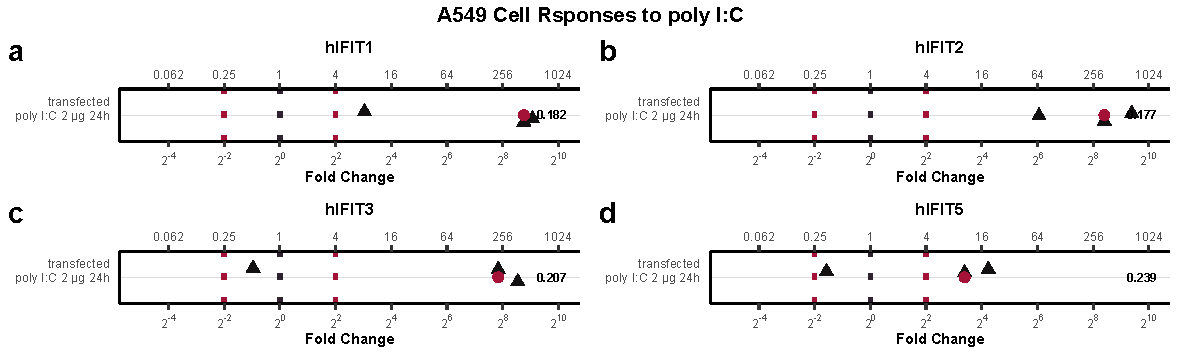
\includegraphics[width=1\linewidth]{06. Chapter 1/Figs/01. Induction/04. a549_treat_polyic.pdf}
    \caption[qPCR Analysis of A549 \textit{hIFIT} Response to Transfected poly I:C.]{\textbf{qPCR Analysis of A549 \textit{hIFIT} Response to Transfected poly I:C.} The relative abundance of (a) \textit{hIFIT1}, (b) \textit{hIFIT2}, (c) \textit{hIFIT3}, and (d) \textit{hIFIT5} genes, extracted from the A549 cell line. The cells were transfected with 2 \(\mu\)g of poly I:C for 24 hours. The shown values are relative to standardised mock values. The red circles signify median values. The black dotted line indicates mock expression, while the red dotted lines indicate biologically significant levels of induction. Numeric values signify the p-values compared to mock.}
    \label{A549 Response to poly I:C}
\end{figure}

When A549 cells were transfected with 2\(\mu\)g of poly I:C for 24 hours we were able to observe the biggest induction compared to the other inducers previously used (Figure \ref{A549 Response to poly I:C}). As with the other inducers, hIFIT1 induction is the greatest (circa 500-fold), followed by \textit{hIFIT2} and \textit{hIFIT3} with 300-fold and 200-fold responses respectively, with \textit{hIFIT5} trailing behind with the lowest response of only 10-fold. This again suggests that \textit{hIFIT5} seems to have differential transcriptomic regulation compared to the other genes of the \textit{IFIT} family. All \textit{hIFIT} values had normal distributions and unequal variance.

\begin{figure}
    \centering
    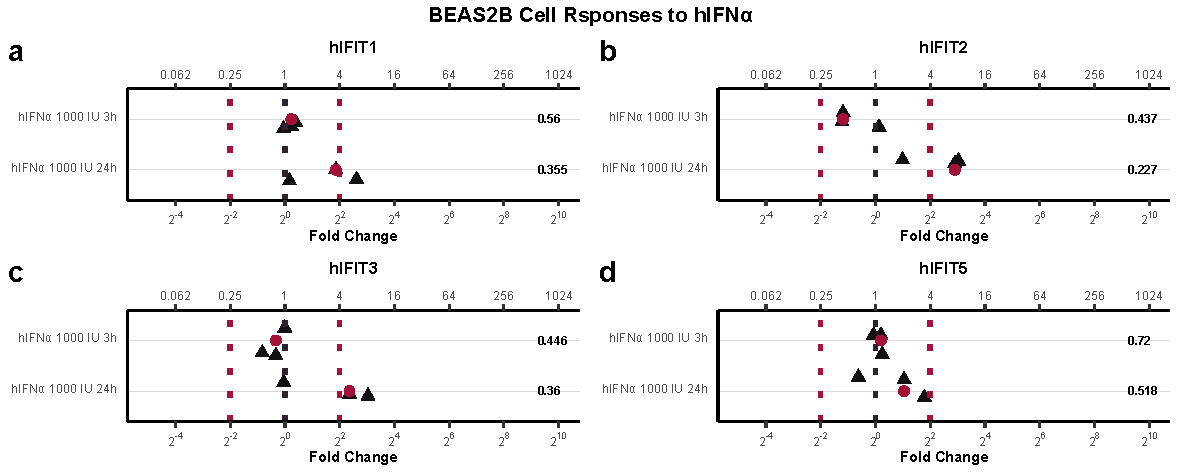
\includegraphics[width=1\linewidth]{06. Chapter 1/Figs/01. Induction/09. beas2b_ifna.pdf}
    \caption[BEAS-2B responses to hIFNa.]{\textbf{BEAS-2B responses to hIFNa.} Text text text text text.}
    \label{BEAS-2B responses to hIFNa.}
\end{figure}

Lastly, we validated the human interferon alpha induction data in a more biologically relevant cell line, BEAS-2B. This is some bronchial cell line or something, I don't know what else to say, I guess something smart and then put a reference in the end (reference for what I said)

\begin{figure}
    \centering
    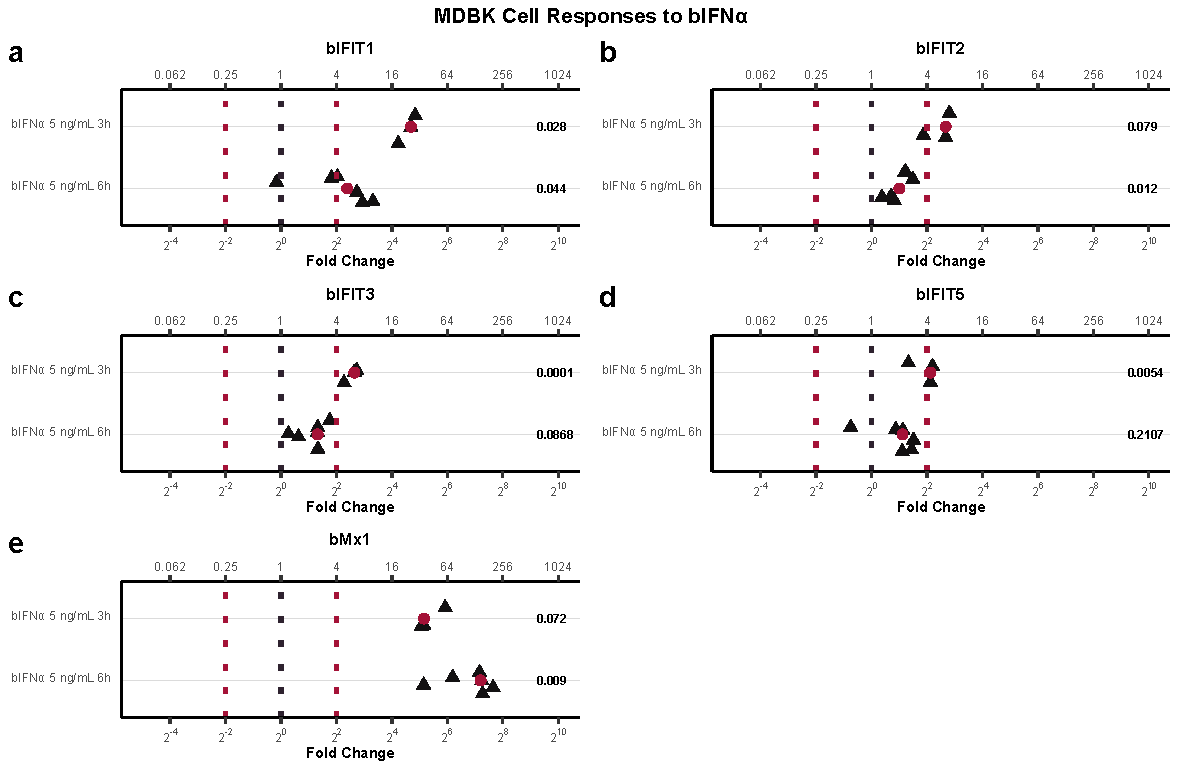
\includegraphics[width=1\linewidth]{07. Chapter 2/Figs/02. Induction/01. mdbk_treat_bifna.pdf}
    \caption[MDBK responses to bIFNa.]{\textbf{MDBK responses to bIFNa.} interferon!!!!!!!!!!}
    \label{MDBK responses to bIFNa}
\end{figure}

The Madin-Darby bovine kidney (MDBK) cell line, derived from bovine renal epithelium in 1958 (Madin and Darby, 1958), is an established model system used in bovine virology studies. In order to assess the bIFIT induction potential in these cells, we have treated the cells with ranging concentrations of known activators of the innate immune system.

As shown in Figure 6, the basal levels of the different bovine IFITs range quite widely. bIFIT1 was detected around the assay detection limit, with bIFIT2 and bIFIT3 having similar values to each other. We detected c. 5000 copies of bIFIT5 per 0.5 µg of RNA under basal conditions. bIFIT1 and bIFIT2 seem not to be induced by LPS, regardless of the concentration, whereas bIFIT3 and especially bIFIT5 responded in a concentration-dependant manner. For all the bIFITs, 0.5 ng/mL of bIFNα was able to cause induction. This was most significant for bIFIT1 which was induced 100-fold. This data confirms the notion that IFITs expression is minimal in unstimulated cells, however, interferon treatment causes their induction even at low concentration. This suggests that bIFNα could be a suitable candidate for positive control of bIFIT induction, although the rest of its concentration range should be assessed as well.

\begin{figure}
    \centering
    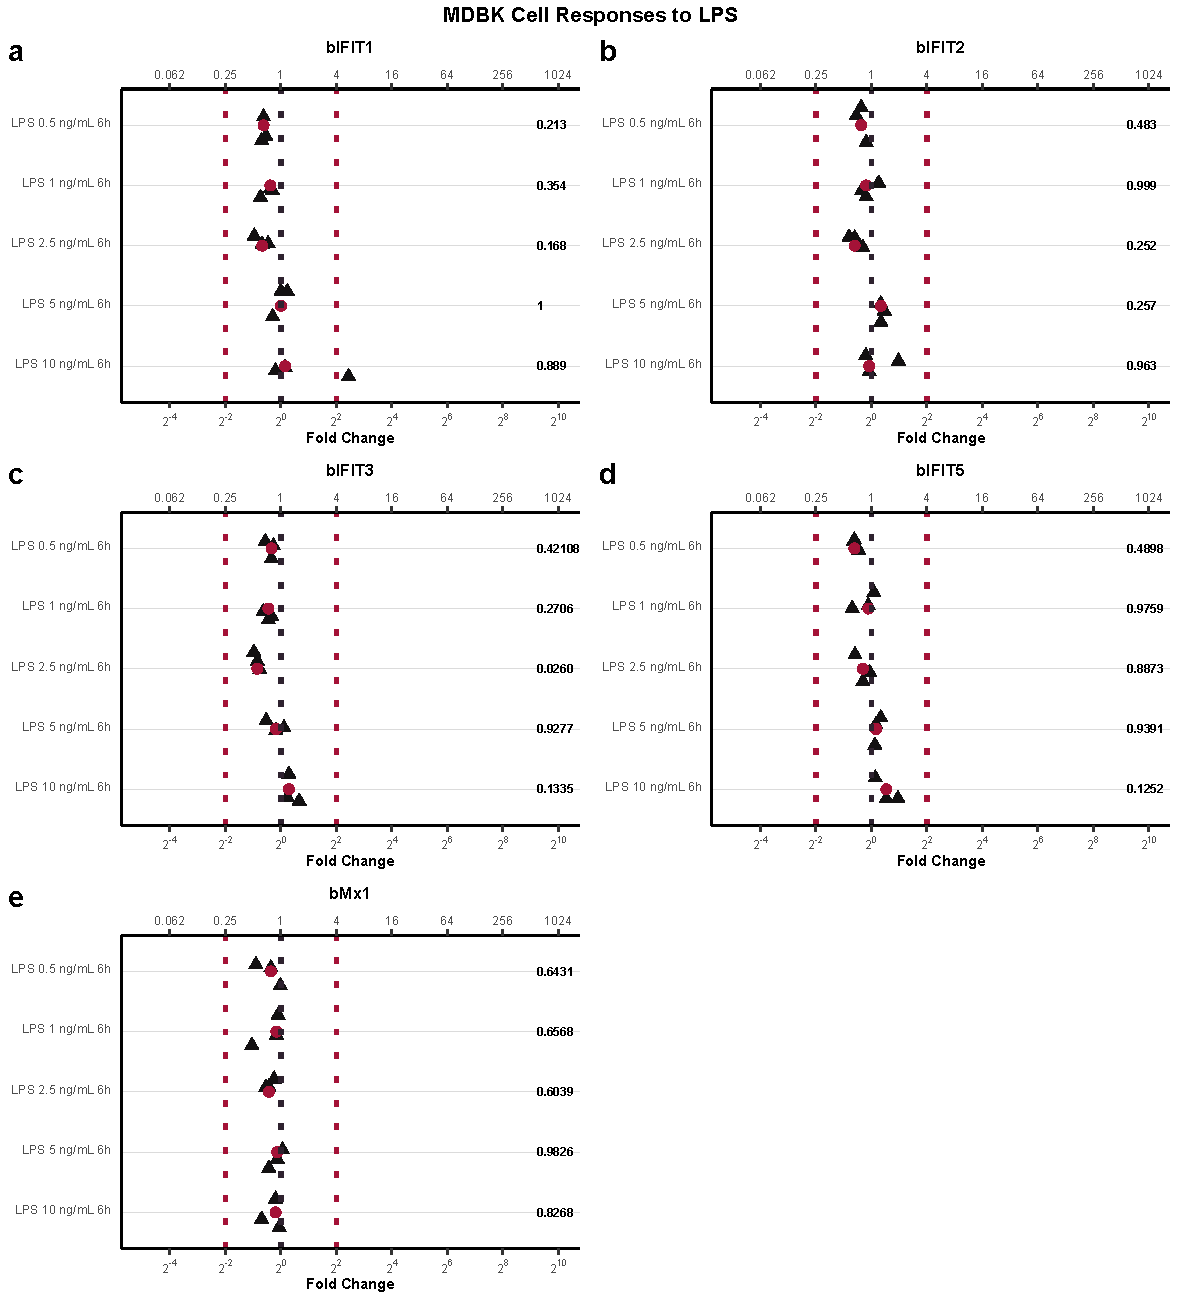
\includegraphics[width=1\linewidth]{07. Chapter 2/Figs/02. Induction/02. mdbk_treat_lps.pdf}
    \caption[MDBK responses to LPS.]{\textbf{MDBK responses to LPS.} lpss!!!!!!!!!!}
    \label{MDBK responses to LPS}
\end{figure}

Bovine Mx1 is included in all experiments with bovine cells as it is an ISG that is induced by range of infections and the activators of innate immune response. It is also a control for bIFN alpha (if it works properly and is not degraded).

Neither bMx1 nor bIFITs are induced by LPS in the concentration range tested. bMx1 was induced by all bIFN alpha at different concentrations and timepoints, but at 5 ng/mL for 24h. This means that either that treatment failed or 24h post adding the bIFN treatment is too late to capture the ISG induction. All targets are induced by bIFN alpha treatment at 5 ng/mL for 3 hours. bIFIT1 also responds to low concentration (0.5 ng/mL) for 6h treatment, but not the other IFITs. No other concentration/time combination induced bIFITs. 

This all suggests that MDBK are responsive to bIFN alpha and capable of bIFIT induction, but the responses are week, especially compared to human cells.

I have a hypothesis that in bovine cells the IFITs are basally expressed to higher levels  (that would explain why we can detect them by IF in mock and infected cell although the qPCR data suggest there is no induction).











\subsubsection{Species-Specific Responses of \textit{IFITs} to RSV} \label{Species-Specific Responses of IFITs to RSV}

\myparagraph{Growth curves of bovine RSV in bovine cell lines} \label{Growth curves of bovine RSV in bovine cell lines}
Describe data: \newline
asdasdasd \newline
This was done as a complement to existing data done by other people in Dalan’s group on human cell lines with hRSV growth curves. The novelty is especially growth curves in BT cells. I do not know if I totally knew what I was doing at the time, so I do not know how much to trust this data.  

\begin{figure}
    \centering
    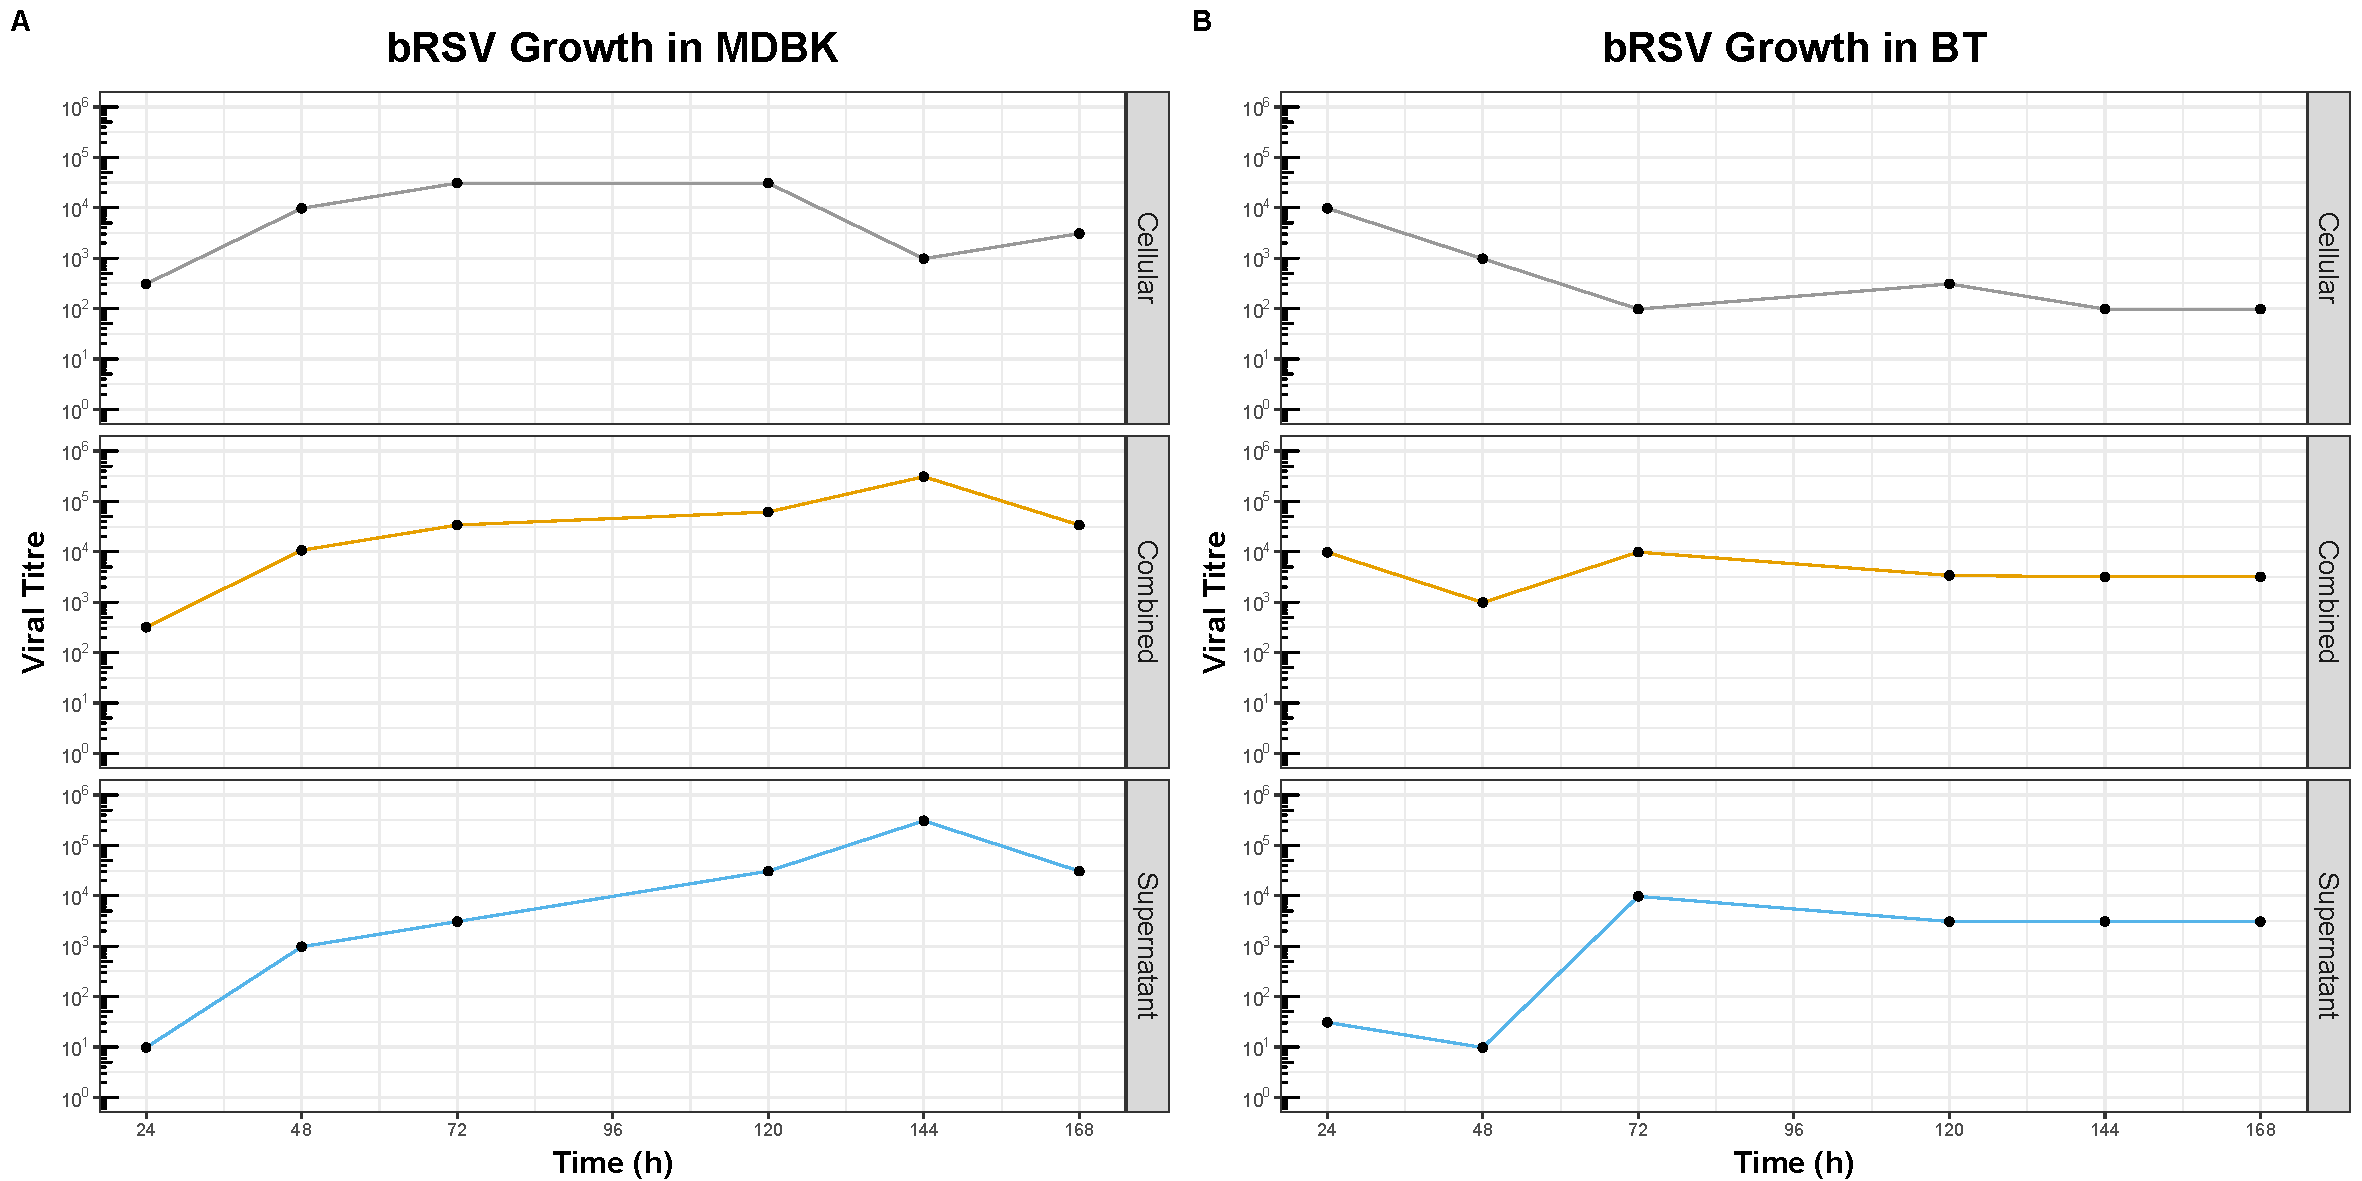
\includegraphics[width=1\linewidth]{07. Chapter 2/Figs/01. Technologies/01. growth_curves.pdf}
    \caption[bRSV growth curves in MDBK and BT cell lines.]{\textbf{bRSV growth curves in MDBK and BT cell lines.} sdfgsdfg sdfg sdfg sdfg sdfg sdfg }
    \label{bRSV growth curves in MDBK and BT cell lines}
\end{figure}


Old text:
In line with bovine IFIT responses investigation, human IFIT responses to human (h) RSV were assessed. The virus was prepared as described in section 7.1. Briefly, infected cells were sonicated, cell debris was separated by centrifugation and virus-containing supernatant was gathered and titred. Human epithelial type 2 (HEp-2) cells were infected with the hRSV-containing supernatant at multiplicities of infection (MOI) of 0.1 and 2. These cells were chosen for the initial preliminary experiments as they are known to grow the virus well and their tissue of origin (laryngeal carcinoma) is relevant to the native site of RSV replication. It is to be noted that this cell line is believed to be contaminated by HeLa cell line and in later experiments should be replaced by more physiological models of human lung epithelial tissue. As a positive control, 1000 U of hIFNα was used. Samples were collected 24 hours post-infection. Cellular RNA was extracted and converted to complementary DNA, as described in section 7.3. Human IFIT transcripts were quantified relative to mock-infected cells. GAPDH-normalised qPCR data can be seen in Figure 8. We observed no significant IFIT induction at the MOI of 0.1, however, infection with hRSV at an MOI of 2 provided significant induction for all targets tested. All human IFITs were induced by approximately 5-fold. With regards to interferon responses, all four targets were transcriptionally upregulated following IFNα treatment. The induction of hIFIT2 was equal to the one induced by viral infection at an MOI of 2, while the rest of hIFITs were induced more greatly. Compared to data described in section 8.3 here the variation was minimal and thus the data is more reliable. We can conclude that both interferon-alpha treatment, as well as RSV infection, transcriptionally upregulate human IFITs in HEp-2 cells.

How were viruses harvested and cells infected \newline
Justify moi and timepoints \newline
Justify uv inactivated virus and how it was done \newline

Describe data: \newline
asdasdasd \newline
UV inactivated RSV does not induce IFIT expression, meaning IFITs do not get activated by TLR4 detection of viral particles on the cell surface. Low MOI infection (0.1 MOI) does not induce IFITs. Infection at MOI 1 and 2 induce all IFITs regardless of the length of infection (24 and 48 HPI). The purification methodology for virus extraction (ultra purification on sucrose cushion vs just clearing the cells + supernatant by centrifugation) does not influence IFIT induction.

\begin{figure}
    \centering
    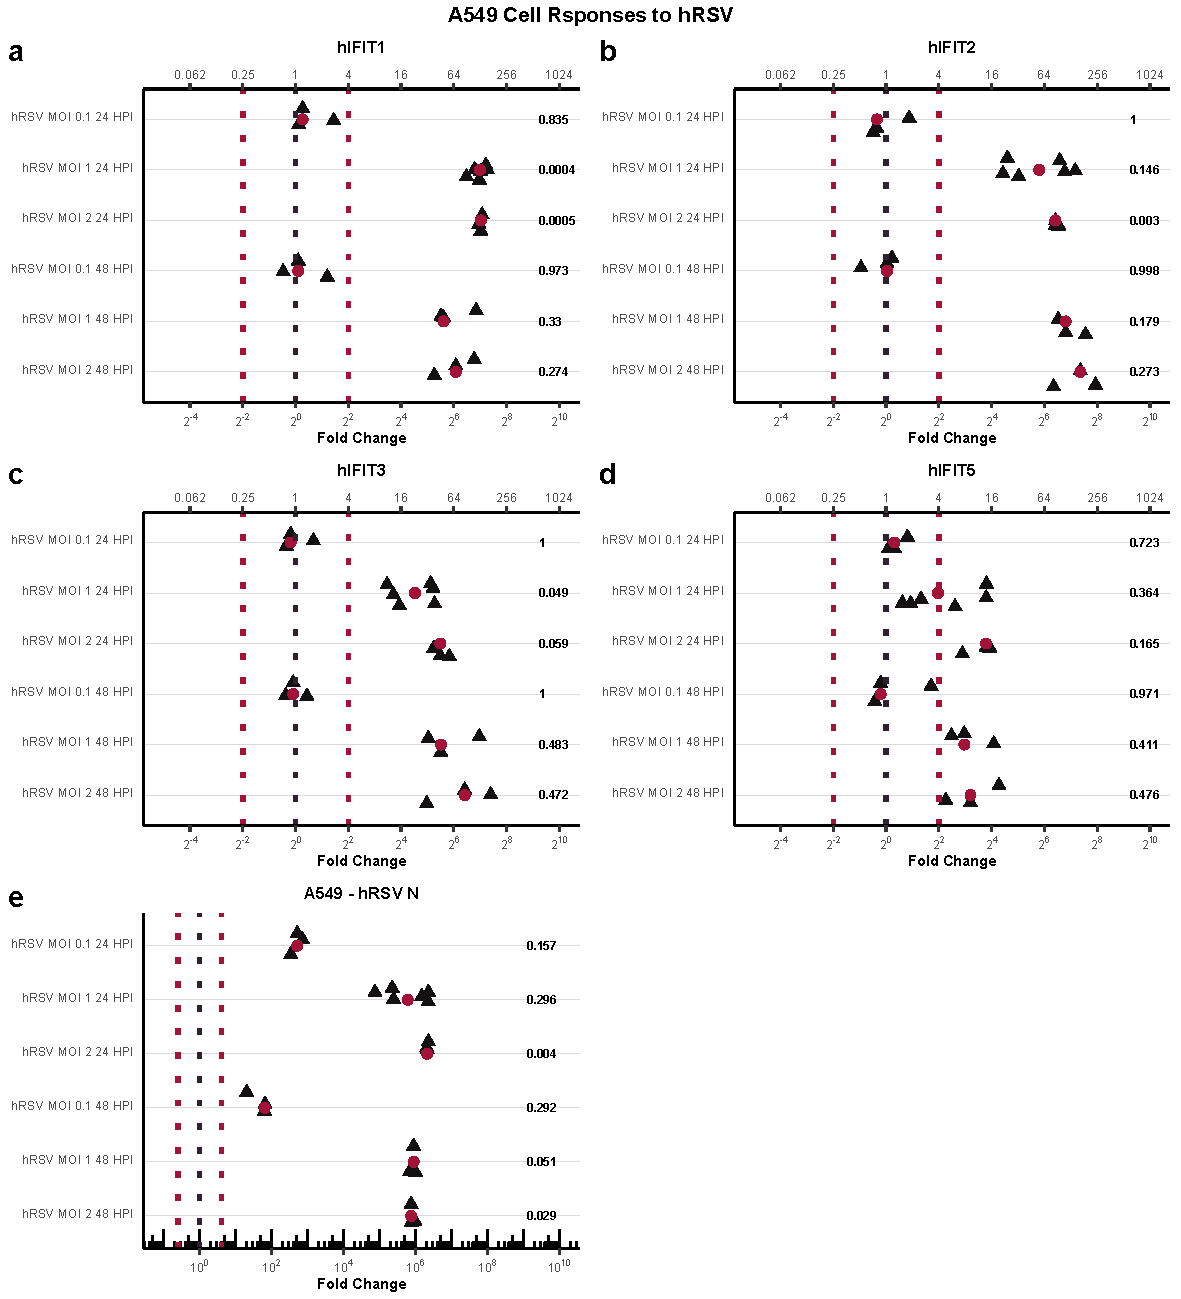
\includegraphics[width=1\linewidth]{06. Chapter 1/Figs/01. Induction/05. a549_hrsv_timepoints.pdf}
    \caption[Responses of A549 to hRSV.]{\textbf{Responses of A549 to hRSV.} Some filler text afterwards.}
    \label{Responses of A549 to hRSV}
\end{figure}

some text between these two suckers that will say about how the human ifit induction is dependent on replication and interferon.

\begin{figure}
    \centering
    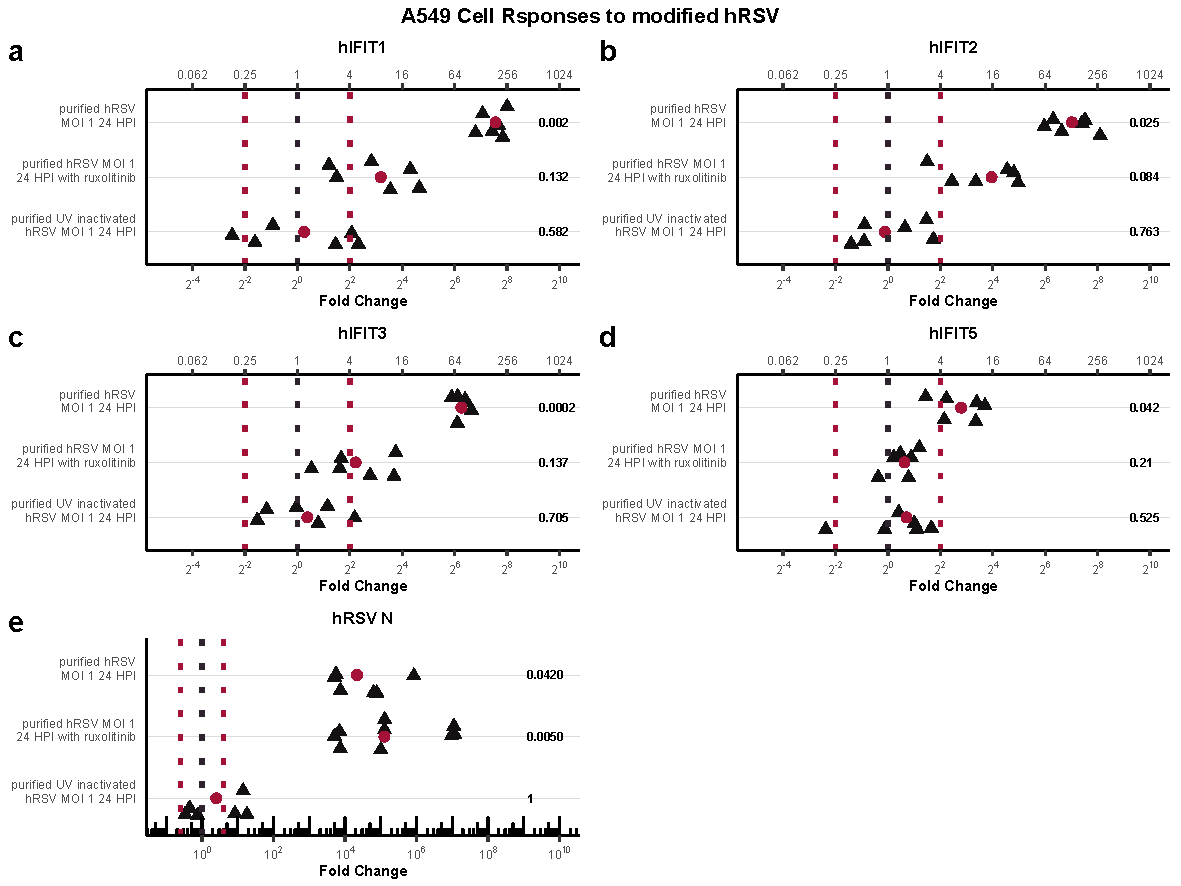
\includegraphics[width=1\linewidth]{06. Chapter 1/Figs/01. Induction/06. a549_hrsv_uv_roxo.pdf}
    \caption[Responses of A549 to modified hRSV.]{\textbf{Responses of A549 to modified hRSV.} Some filler text afterwards.}
    \label{Responses of A549 to modified hRSV.}
\end{figure}

\begin{figure}
    \centering
    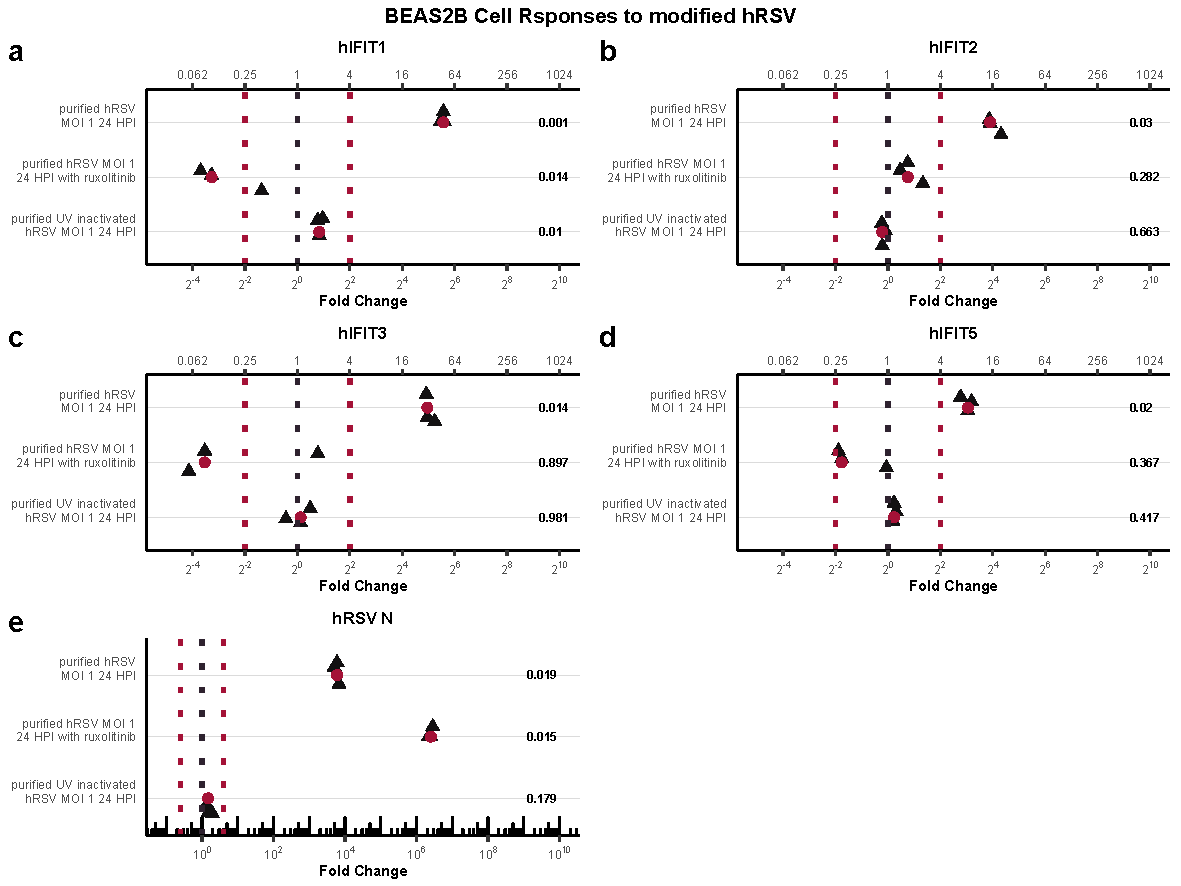
\includegraphics[width=1\linewidth]{06. Chapter 1/Figs/01. Induction/10. beas2b_hrsv.pdf}
    \caption[BEAS-2B responses to hRSV.]{BEAS-2B responses to hRSV.}
    \label{BEAS-2B responses to hRSV.}
\end{figure}



Describe data: \newline
asdasdasd \newline
Validation in more physiologically relevant cell line. UV inactivated hRSV does not cause induction. Ultracentrifugation purified hRSV causes induction in all IFITs. All IFITs but IFIT5 are induced by IFN alpha, but only after incubation for 24 hours (3h incubation does not cause induction). This shows that the cells are interferon competent. IFIT5 does not get induced by any bRSV infection tried (probably because IFIT5 has either basally higher levels and thus the same end mRNA concentration equates to lower induction or because it is really not induced by bRSV (although the IFITs should have the same promoters)). Low MOI infection (0.001 and 0.01) of dNS1 and dNS2 bRSV induces IFITs 1,2 and 3, while dSH MOI1 and dNS1/2 MOI 0.001 does not. 

The trends seen with A549 are kind of recapitulated.


Old text:
Alongside confirming the induction potential of bIFITs in MDBK cells, we assessed the effect of bovine respiratory syncytial virus (bRSV) on IFIT induction. As bRSV is a known inducer of the interferon response we expect bovine IFIT genes to be upregulated following infection. MDBK cells were infected with purified bRSV at MOI of 1 for 24 and 48 hours. As a positive control human IFNα was used. This was due to the unavailability of a bovine counterpart at that point, however, Gresser and his colleagues (1974), reported that hIFNα does indeed affect bovine cells as well. Cellular RNA was extracted and converted to complementary DNA, as described in section 7.3. Bovine IFIT transcripts were quantified relative to mock-infected cells. qPCR results (Figure 7A) were normalised to bovine GAPDH levels. We observed large variation in the transcriptional response, even in mock-infected cells. bIFITs 2, 3 and 5 mRNA levels did not change in response at any time point post bRSV infection. bIFIT1 was induced at 48 hours post-infection, but the variation is too high to make firm conclusions at this point. However, consistent with Gresser et al’s previous findings, bIFITs were responsive to 1000 units of hIFNα; all genes were highly induced (Figure 7B), although the fold expression increases varied greatly. bIFIT1 increased 10000-fold, followed by bIFIT2 and bIFIT3 with both having c. 700-fold increase. bIFIT5 mRNA expression was induced by c. 25-fold after treatment with hIFNα. This experiment was performed once and will be repeated. As a control for infection, quantification of viral RNA using qPCR will provide us with a clearer picture about the observed changes.

Describe data: \newline
asdasdas

UV inactivated bRSV causes no change for bMx1 and bIFIT2 and seems to downregulate bIFIT1,3,5. Low, mid, and high MOI (0.1, 1, 2) and two different time points (24 and 48 HPI) do not seem to influence the levels of any genes tested other than for bMx1 for wt ultracentrifugation purified bRSV 24 HPI MOI 1. I have one experiment where bRSV MOI 1 24 HPI downregulates all genes tested but it might be a technical error. 
Very low MOI (0.001) wt bRSV along with MOI 1 dSH and very low MOI dNS1, dSN2 and dNS1/2 bRSV do not up or downregulate any genes tested in a biologically significant way.

\begin{figure}
    \centering
    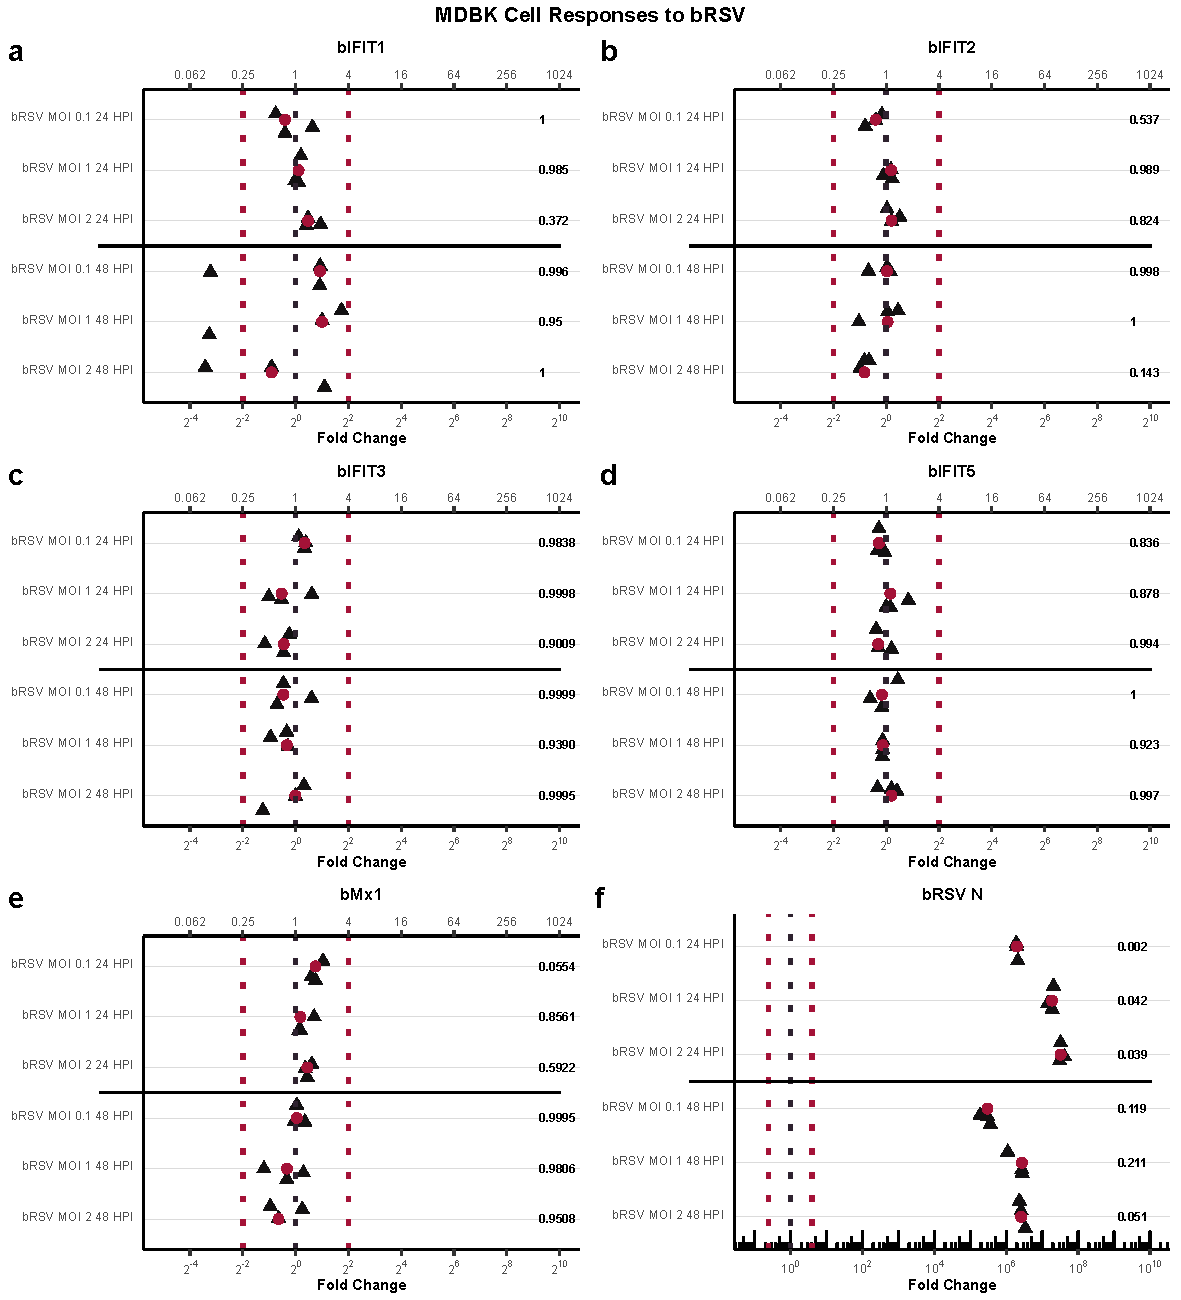
\includegraphics[width=1\linewidth]{07. Chapter 2/Figs/02. Induction/03. mdbk_brsv_timepoints.pdf}
    \caption[MDBK responses to bRSV.]{\textbf{MDBK responses to bRSV.} timepoints infection }
    \label{MDBK responses to bRSV}
\end{figure}

\begin{figure}
    \centering
    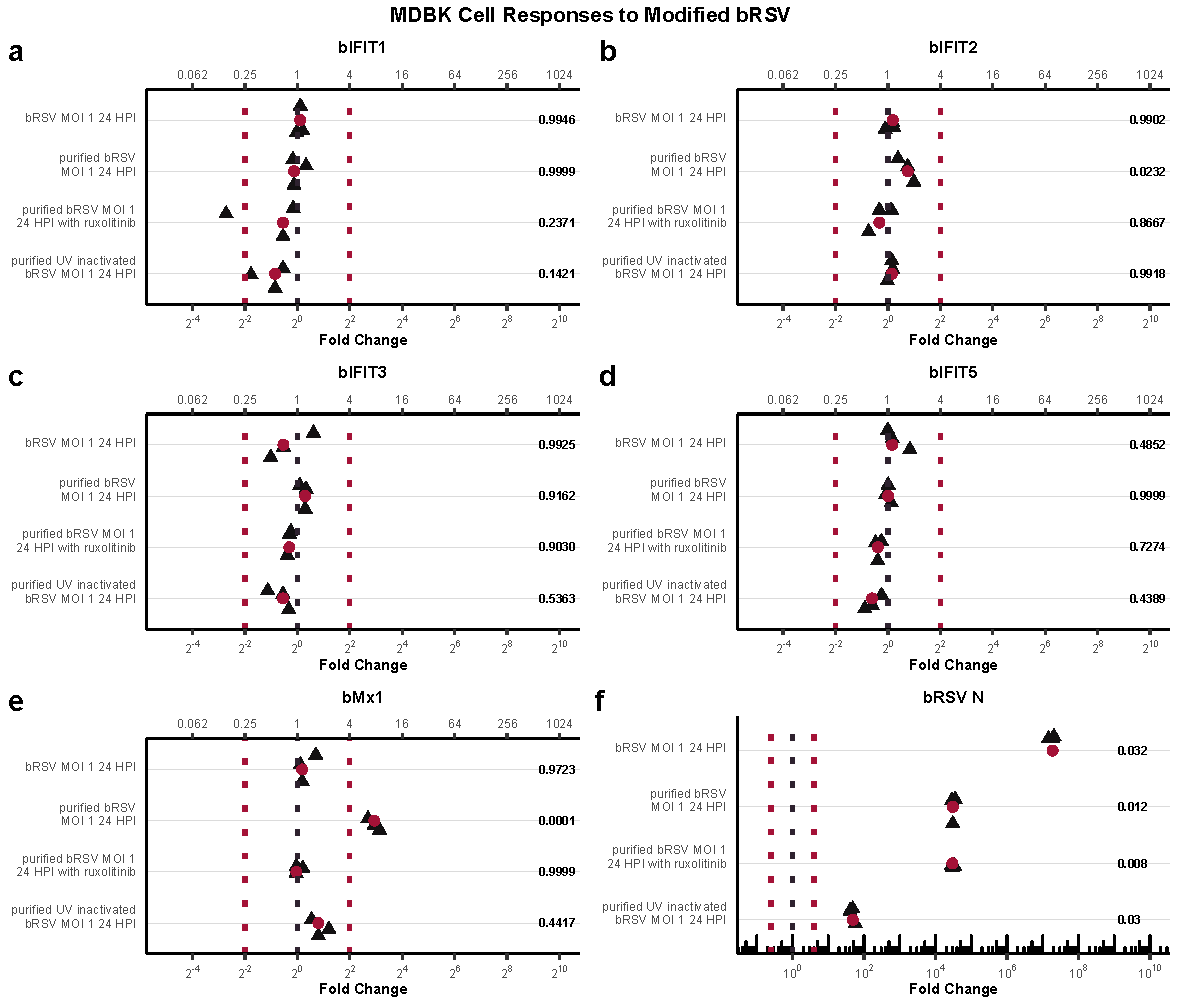
\includegraphics[width=1\linewidth]{07. Chapter 2/Figs/02. Induction/04. mdbk_brsv_uv_roxo.pdf}
    \caption[MDBK responses to modified bRSV.]{\textbf{MDBK responses to modified bRSV.} asdf as asdf asdf asdf as asdf asdf assd }
    \label{MDBK responses to modified bRS}
\end{figure}

\begin{figure}
    \centering
    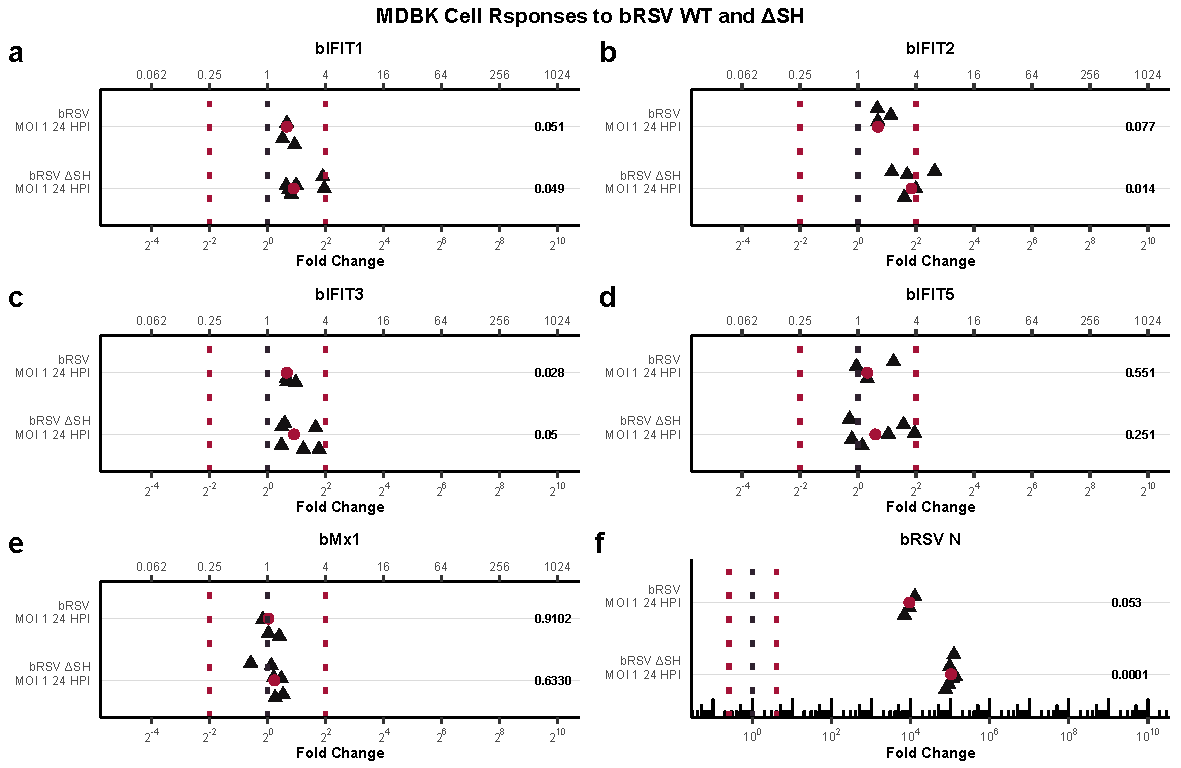
\includegraphics[width=1\linewidth]{07. Chapter 2/Figs/02. Induction/05. mdbk_brsv_moi1_dsh.pdf}
    \caption[MDBK responses to dSH.]{\textbf{MDBK responses to dSH.} timepoints infection }
    \label{MDBK responses to dSH}
\end{figure}

\begin{figure}
    \centering
    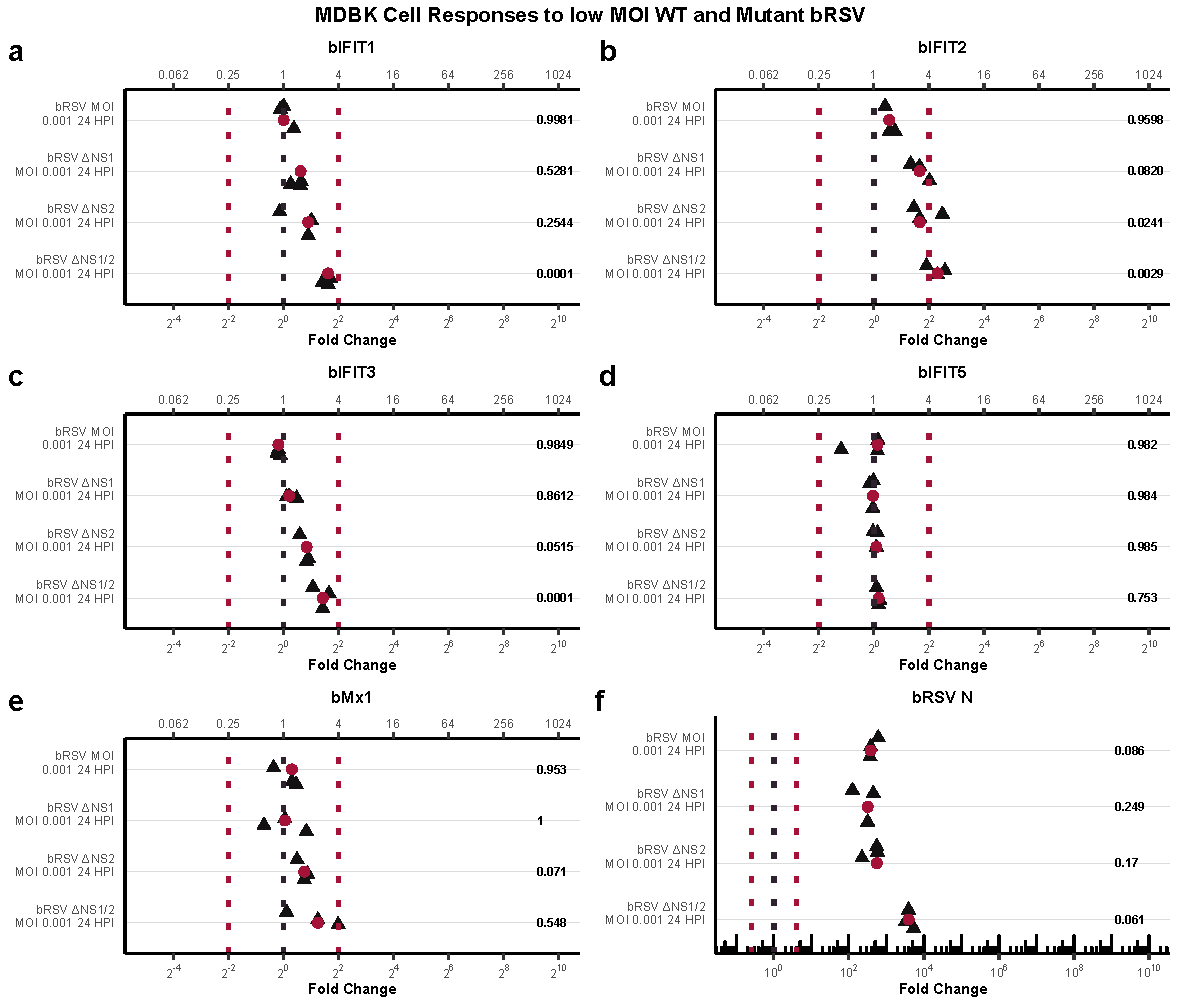
\includegraphics[width=1\linewidth]{07. Chapter 2/Figs/02. Induction/06. mdbk_brsv_low_moi.pdf}
    \caption[MDBK responses to low MOI mutant bRSV.]{\textbf{MDBK responses to low MOI mutant bRSV.} asdf as asdf asdf asdf as asdf asdf assd }
    \label{MDBK responses to low MOI mutant bRSV}
\end{figure}



\subsubsection{Validation in More Physiological Cell Lines} \label{Validation in More Physiological Cell Lines}
Why beas2b \newline
How it was cultured + all treatment the same as in a549












\subsection{Expression of Human and Bovine IFITs} \label{Expression of Human and Bovine IFITs}
\subsubsection{Validation Antibodies} \label{Validation Antibodies}
Overexpressed human IFITs \newline
figures

\begin{figure}
    \centering
    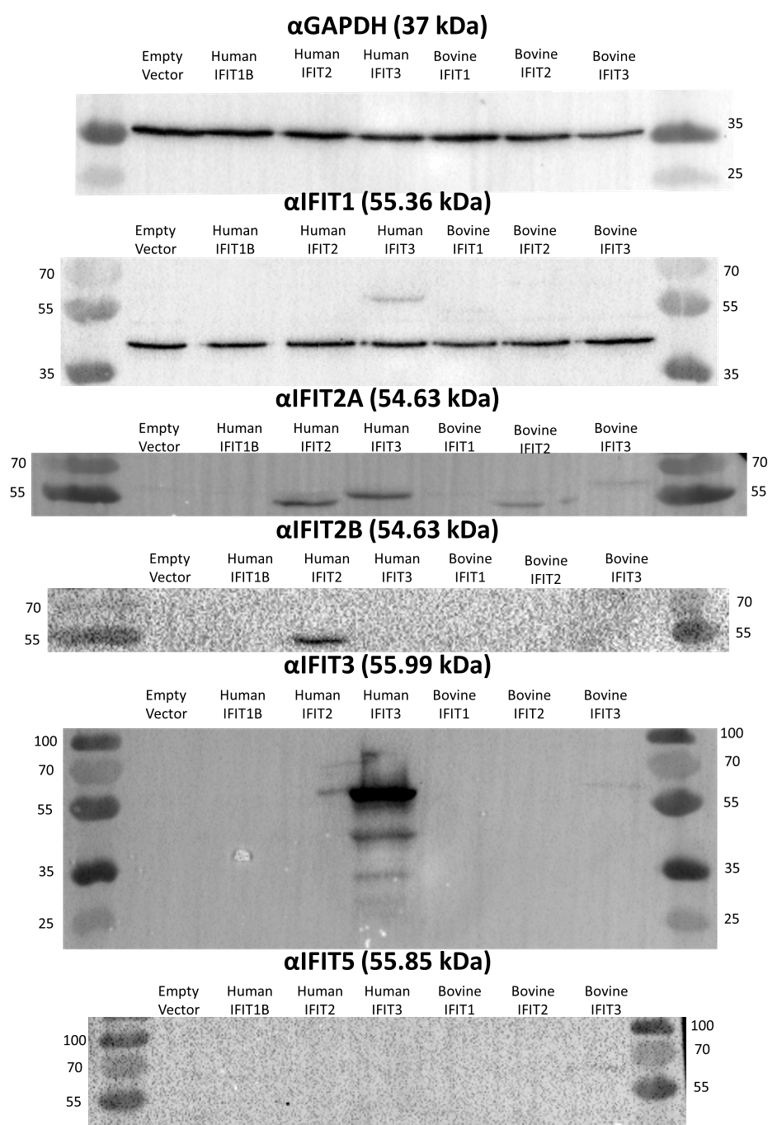
\includegraphics[width=0.5\linewidth]{06. Chapter 1/Figs/02. Expression/01. atb-validation.png}
    \caption[Human IFIT antibody validation.]{\textbf{Human IFIT antibody validation.} test test test test test test test test test test test.}
    \label{Human IFIT antibody validation.} 
\end{figure}

\subsubsection{Western Blots of Treatment and Infection} \label{Western Blots of Treatment and Infection}
Western of time course of treatment with IFN etc. (GAPDH, IFITs) \newline
Western of infection time course (N, P, GAPDH, IFITs) \newline
A549, BEAS2B

\begin{figure}
    \centering
    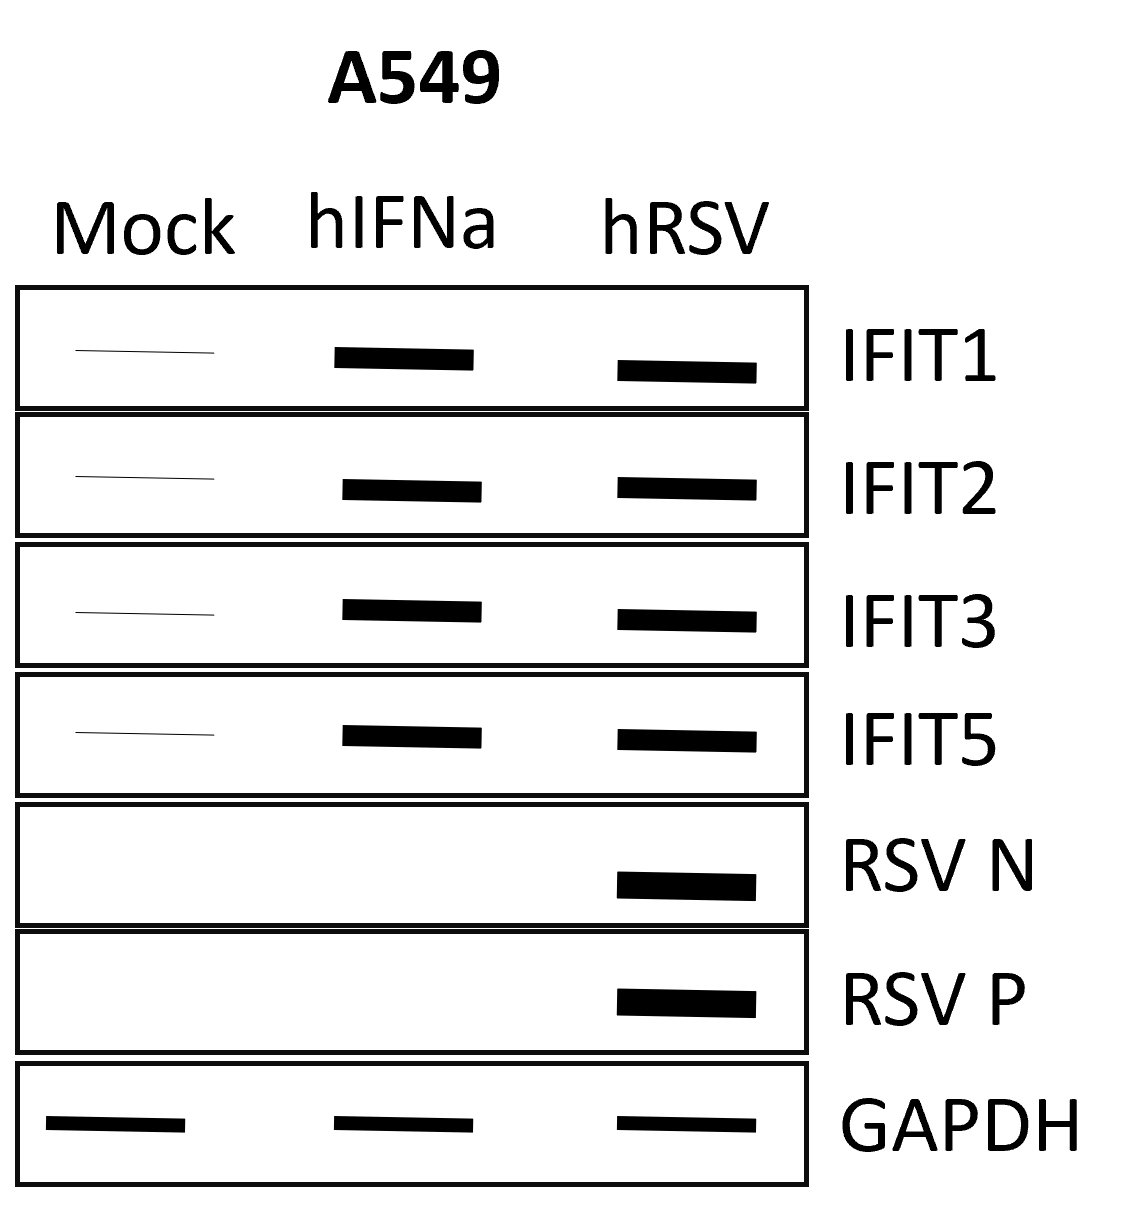
\includegraphics[width=0.5\linewidth]{06. Chapter 1/Figs/02. Expression/02. A549 WB.png}
    \caption[A549 Western Blot.]{\textbf{A549 Western Blot.} test test test test test test test test test test test.}
    \label{A549 Western Blot.}
\end{figure}

\begin{figure}
    \centering
    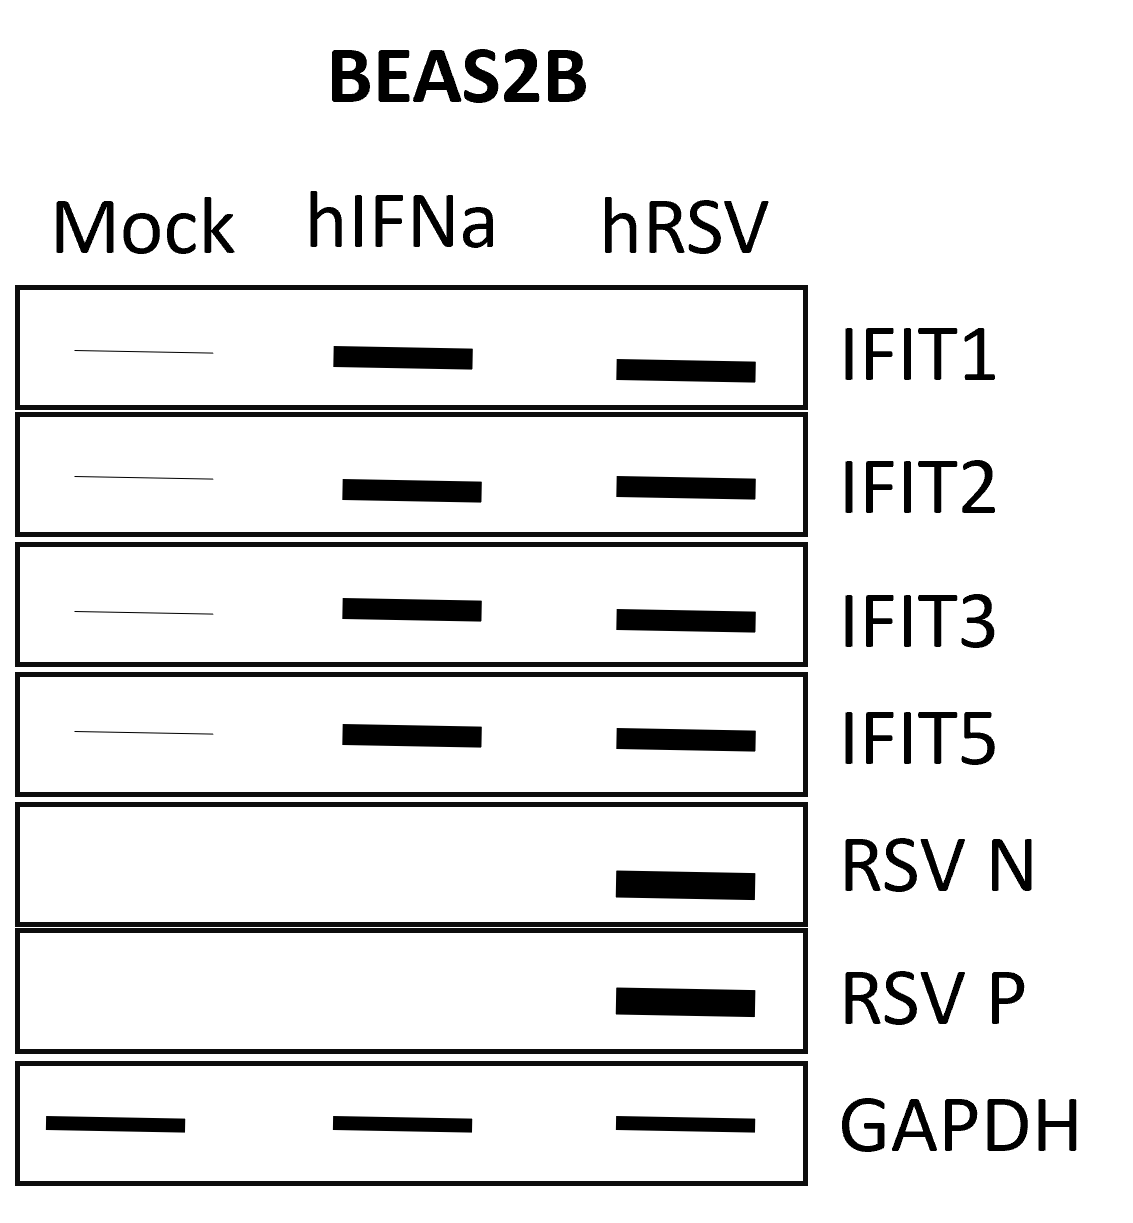
\includegraphics[width=0.5\linewidth]{06. Chapter 1/Figs/02. Expression/03. beas2b wb.png}
    \caption[BEAS-2B Western Blot.]{\textbf{BEAS-2B Western Blot.} test test test test test test test test test test test.}
    \label{BEAS-2B Western Blot.}
\end{figure}

\subsubsection{Validation by Comparing to the Proteomic Dataset} \label{Validation by Comparing to the Proteomic Dataset}
Who, what and why it was done  \newline
Cite the bioArchive paper \cite{Jobe2023ViralCondensates}

\begin{figure}
    \centering
    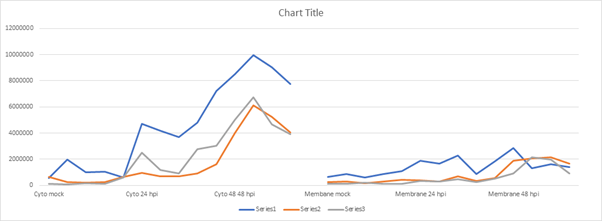
\includegraphics[width=1\linewidth]{06. Chapter 1/Figs/02. Expression/04. proteomics.png}
    \caption[Human IFIT proteins detected per fraction.]{\textbf{Human IFIT proteins detected per fraction.} test test test test test test test test test test test.}
    \label{Human IFIT proteins detected per fraction.}
\end{figure}

Describe data: \newline
asdasdasd \newline
Proteomics dataset from Dalan’s lab looking at differential enrichment of proteins between membrane and cytosolic fractures. It confirms that in A549 (I think) IFITs 1 (series 1), 2 (series 2) and 3 (series 3) are induced in the cytosolic fraction at protein level 







\subsubsection{Western Blots of Treatment and Infection} \label{Western Blots of Treatment and Infection}
Western of time course of treatment with IFN etc. (GAPDH, IFITs) \newline
Western of infection time course (N, P, GAPDH, IFITs) \newline
MDBK, BT

\begin{figure}
    \centering
    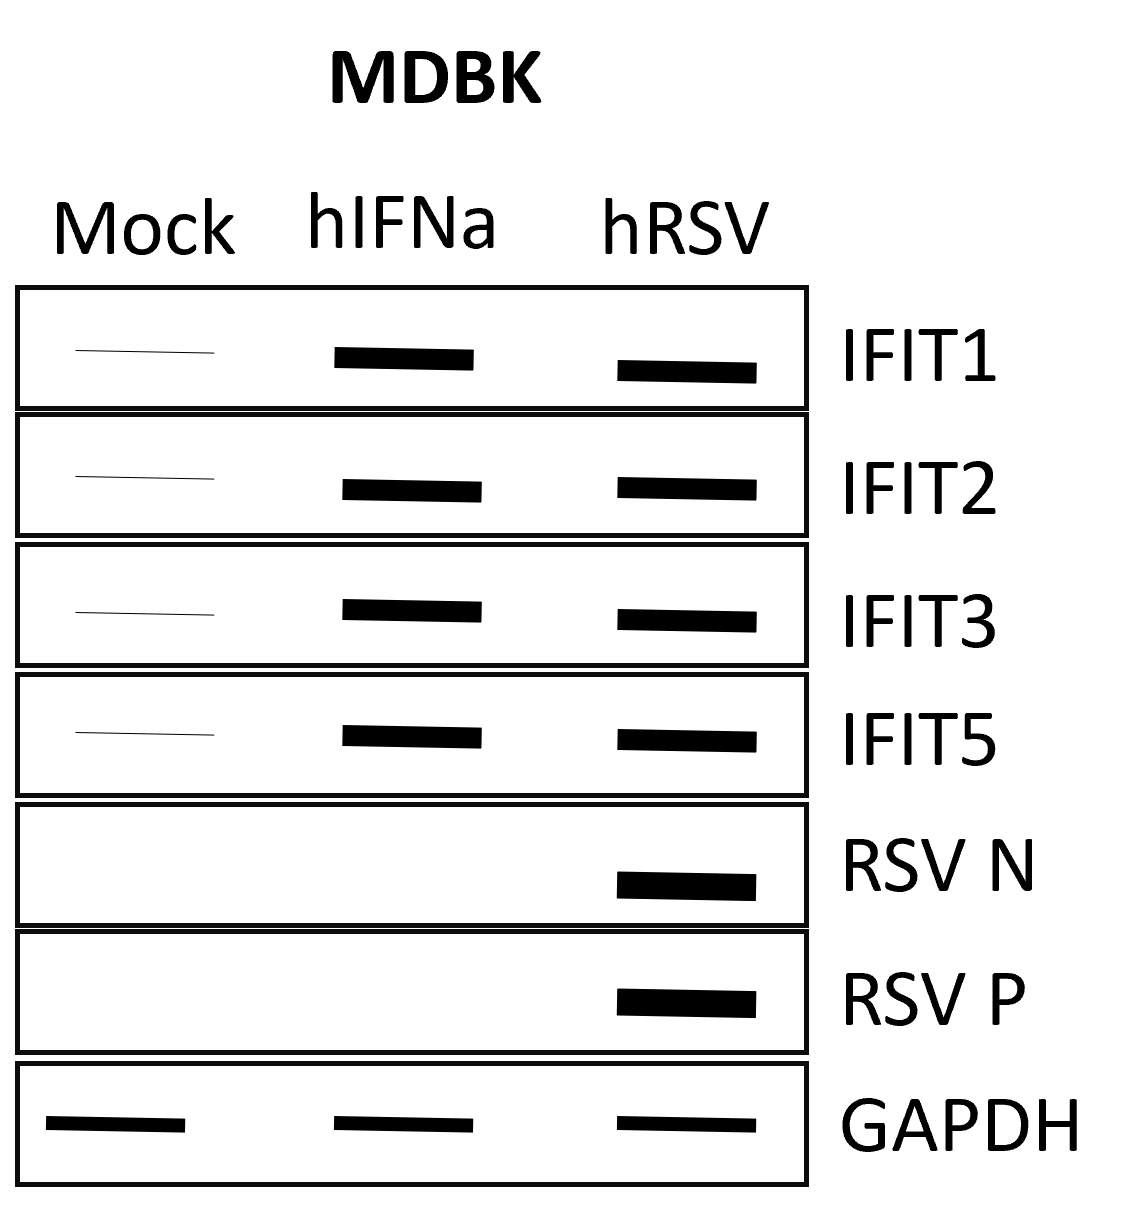
\includegraphics[width=0.5\linewidth]{07. Chapter 2/Figs/03. Expression/02. mdbk wb.png}
    \caption[MDBK Western Blot.]{\textbf{MDBK Western Blot.} test test test test test test test test test test test.}
    \label{MDBK Western Blot.}
\end{figure}

\begin{figure}
    \centering
    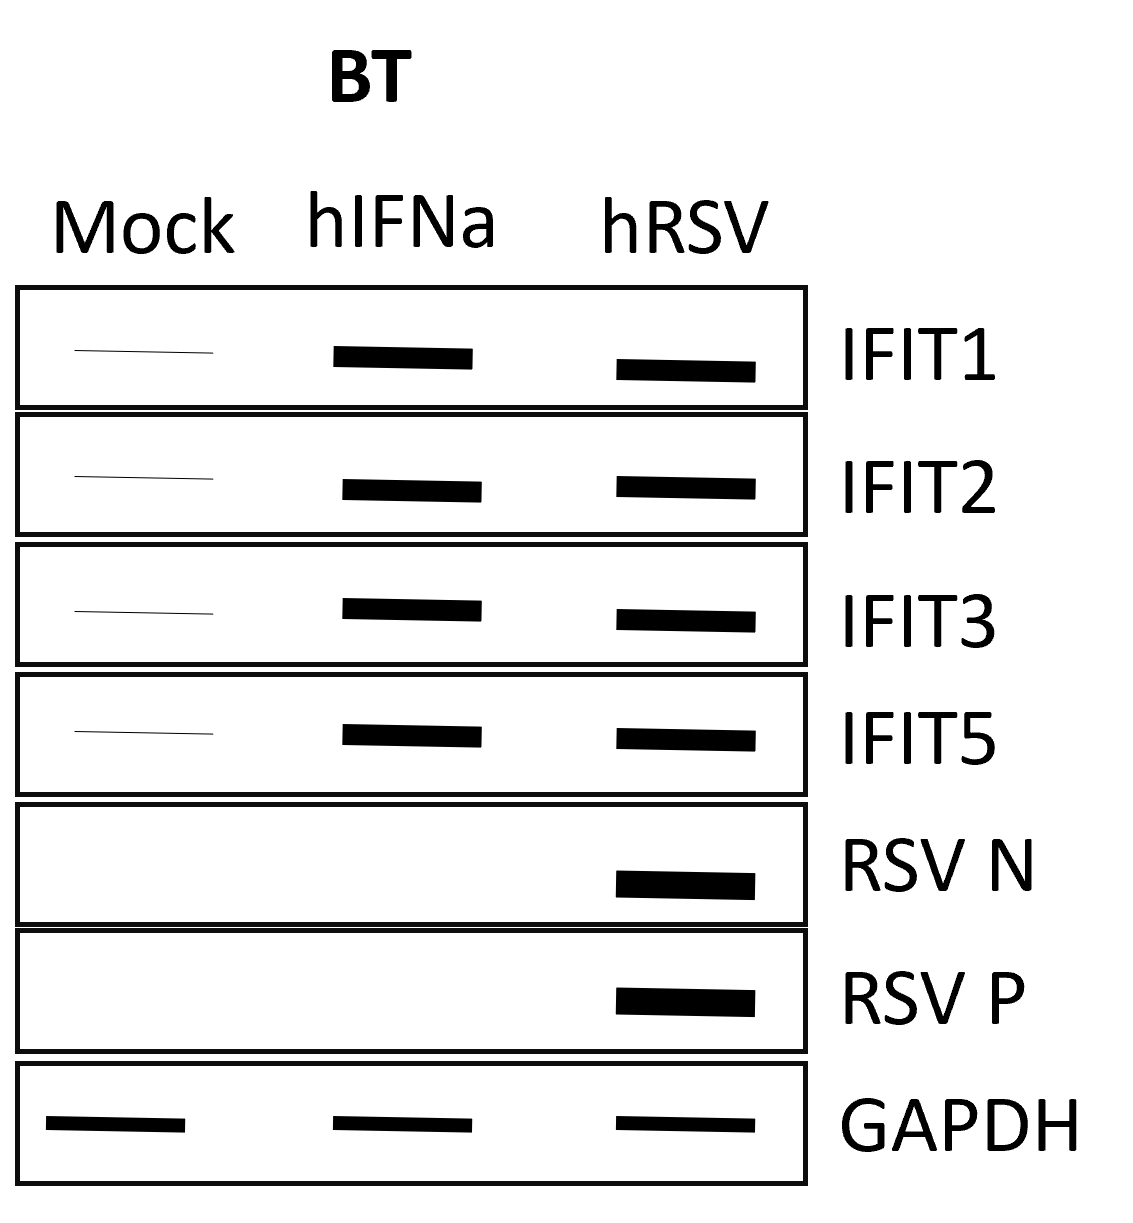
\includegraphics[width=0.5\linewidth]{07. Chapter 2/Figs/03. Expression/03. bt wb.png}
    \caption[BT Western Blot.]{\textbf{BT Western Blot.} test test test test test test test test test test test.}
    \label{BT Western Blot.}
\end{figure}

\subsection{Localisation of Human and Bovine IFITs} \label{Localisation of Human and Bovine IFITs}
Asdfasfsdfasdf \newline
IF Mock | INF | Infection \newline
A549 BEAS2B

Merge pictures of clusters of cells looking at changes between subcellular localisation and a clear increase in mean intensity. Graphs show mean intensity changes from all cells imaged.

\begin{figure}
    \centering
    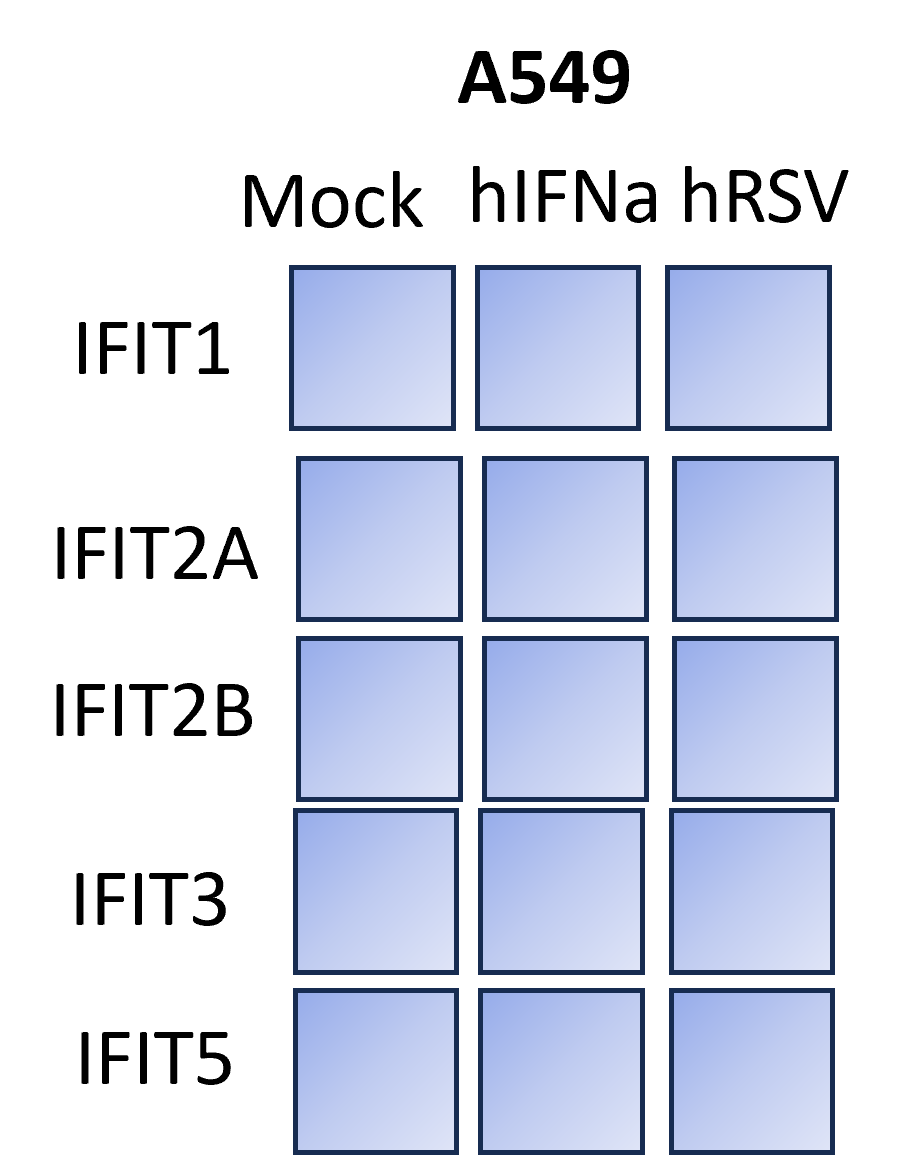
\includegraphics[width=1\linewidth]{06. Chapter 1/Figs/03. Localisation/01. a549 merges.png}
    \caption[A549 localisation mergers.]{A549 localisation mergers.}
    \label{A549 localisation mergers.}
\end{figure}


\begin{figure}
    \centering
    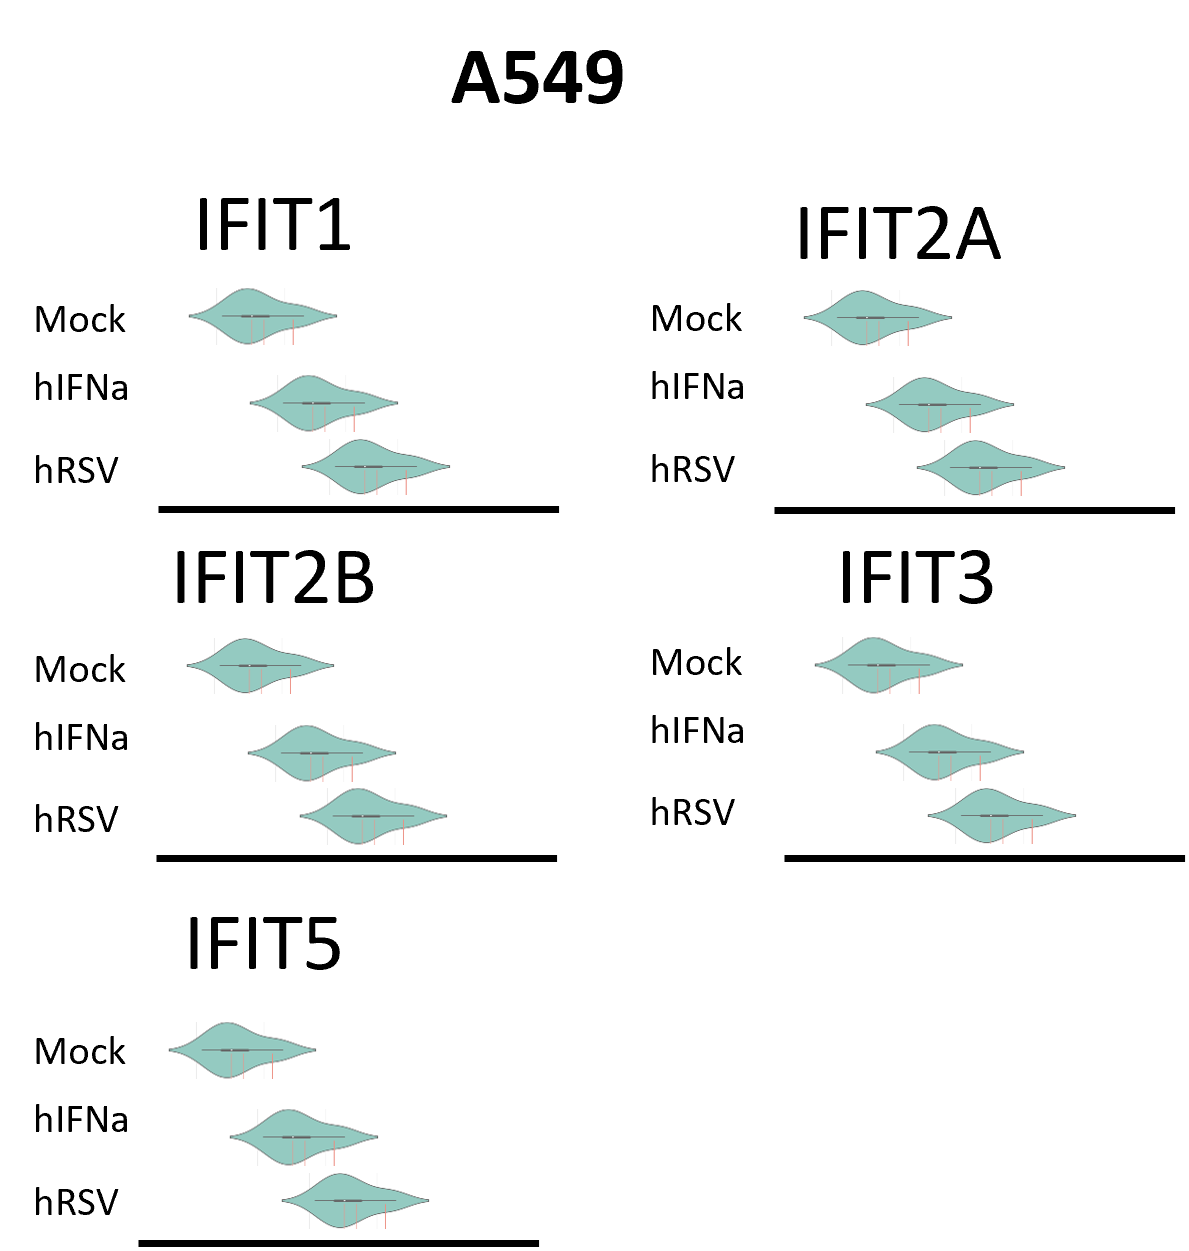
\includegraphics[width=1\linewidth]{06. Chapter 1/Figs/03. Localisation/02. a549 plots.png}
    \caption[A549 localisation plots.]{A549 localisation plots.}
    \label{A549 localisation plots.}
\end{figure}


\begin{figure}
    \centering
    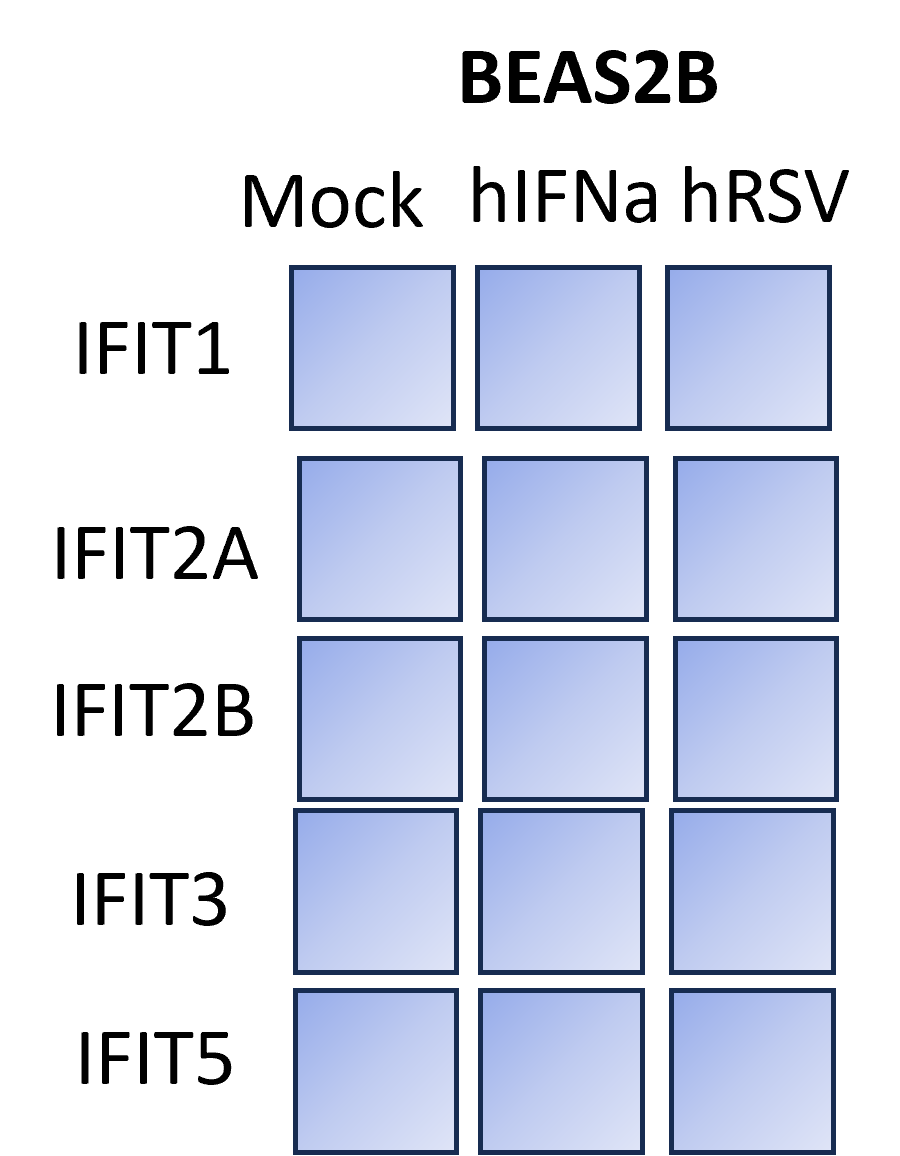
\includegraphics[width=1\linewidth]{06. Chapter 1/Figs/03. Localisation/03. beas2b merges.png}
    \caption[BEAS-2B localisation mergers.]{BEAS-2B localisation mergers.}
    \label{BEAS-2B localisation mergers.}
\end{figure}


\begin{figure}
    \centering
    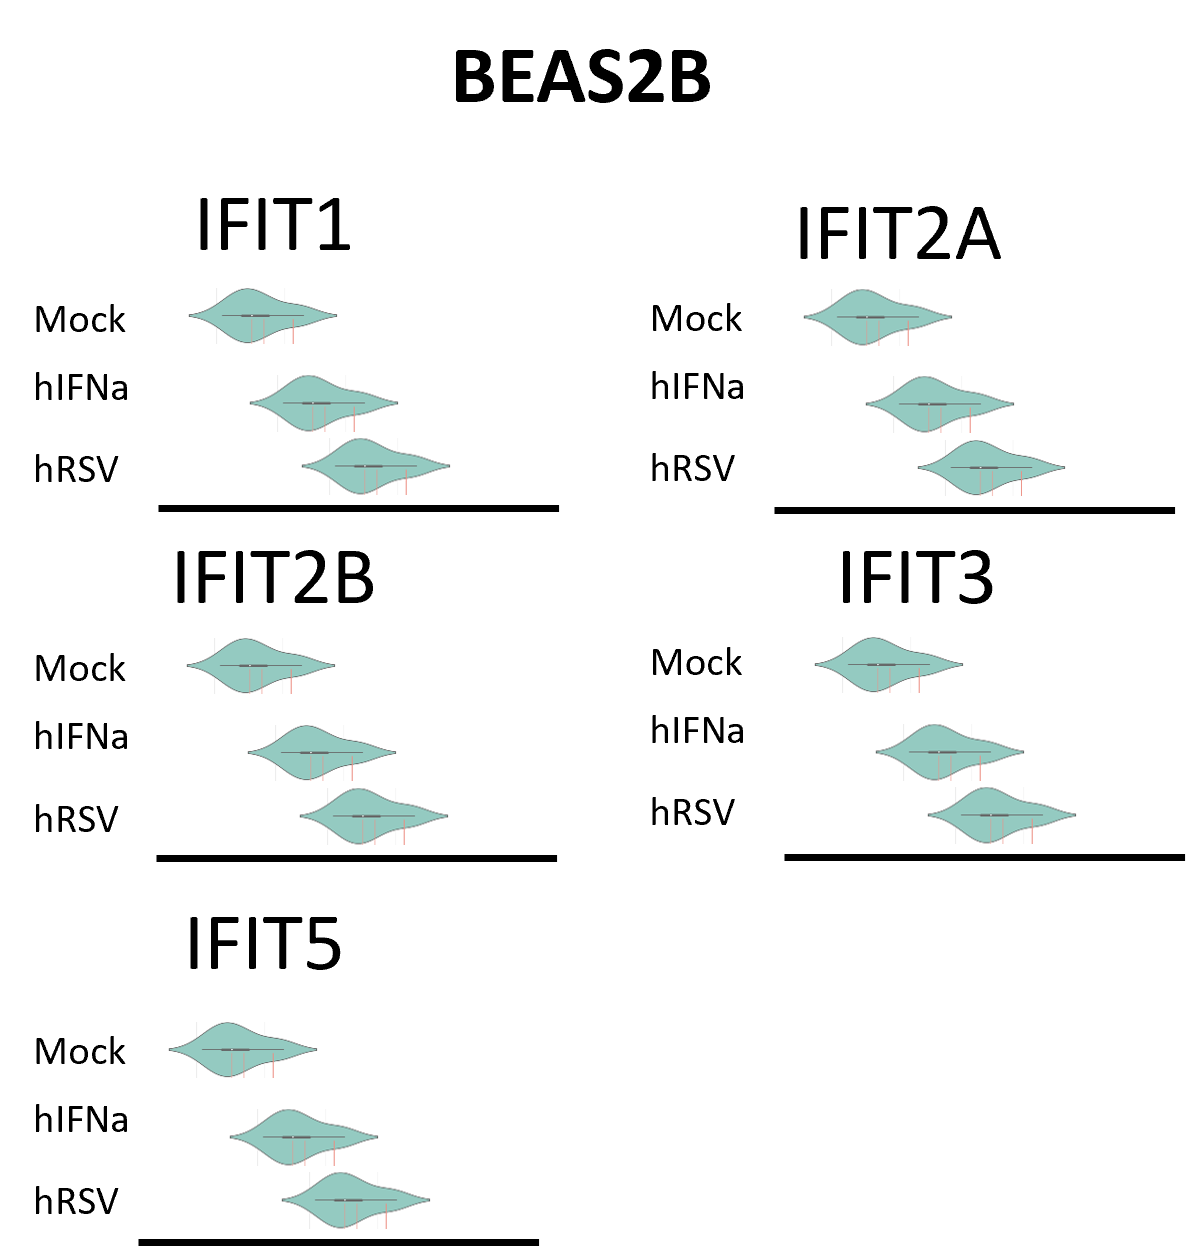
\includegraphics[width=1\linewidth]{06. Chapter 1/Figs/03. Localisation/04. beas2b plots.png}
    \caption[BEAS-2B localisation plots.]{BEAS-2B localisation plots.}
    \label{BEAS-2B localisation plots.}
\end{figure}



\subsection{Localisation of bovine IFITs}
Asdfasfsdfasdf \newline
IF Mock | INF | Infection | Roxo \newline
MDBK BT

Merge pictures of clusters of cells looking at changes between subcellular localisation and a clear increase in mean intensity. Graphs show mean intensity changes from all cells imaged.

\begin{figure}
    \centering
    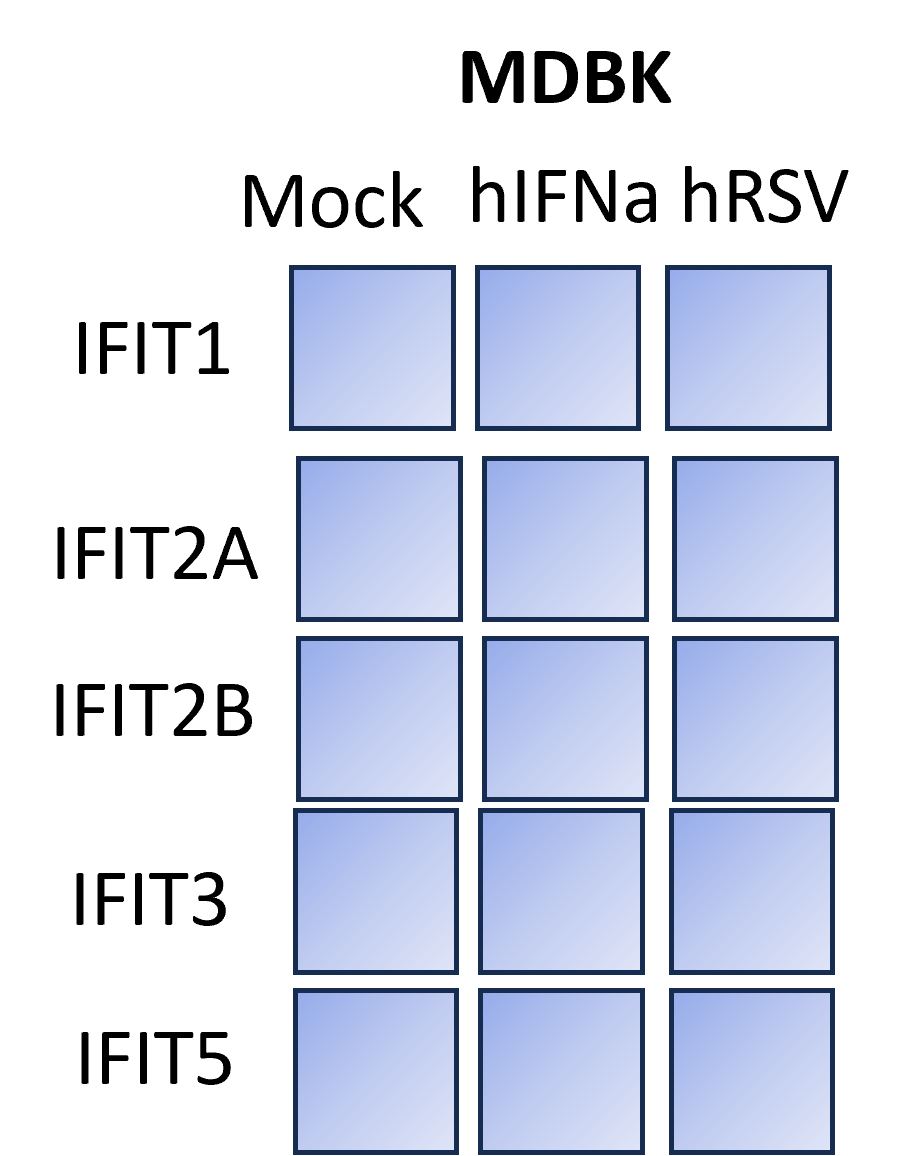
\includegraphics[width=1\linewidth]{07. Chapter 2/Figs/04. Localisation/01. mdbk merges.png}
    \caption[MDBK localisation mergers.]{MDBK localisation mergers.}
    \label{MDBK localisation mergers.}
\end{figure}


\begin{figure}
    \centering
    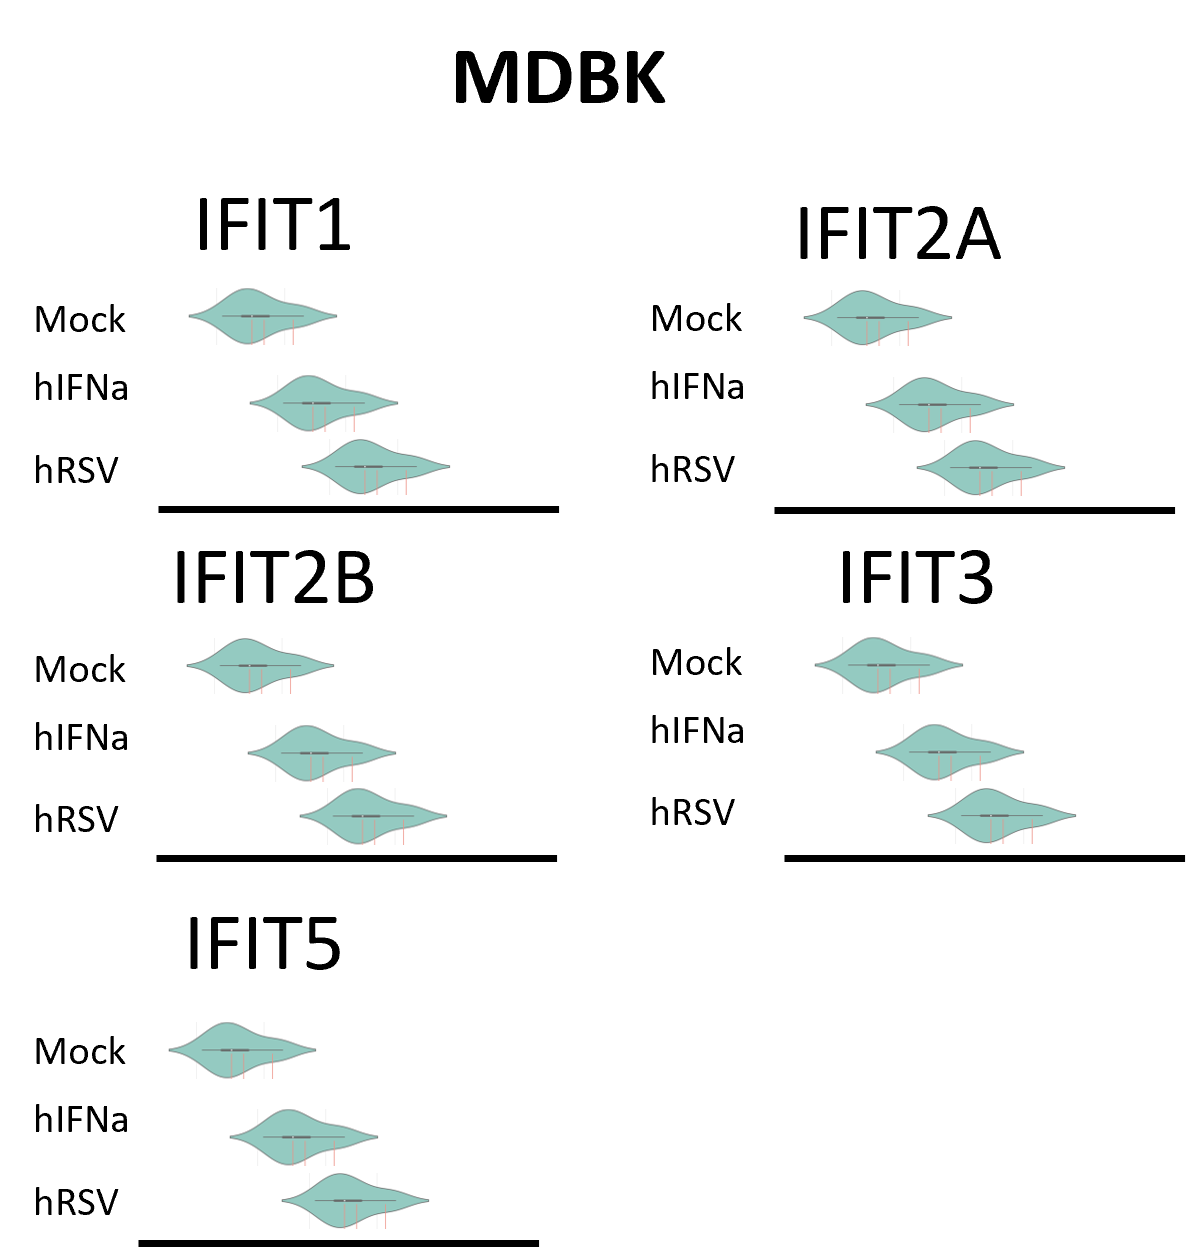
\includegraphics[width=1\linewidth]{07. Chapter 2/Figs/04. Localisation/02. mdbk plots.png}
    \caption[MDBK localisation plots.]{MDBK localisation plots.}
    \label{MDBK localisation plots.}
\end{figure}


\begin{figure}
    \centering
    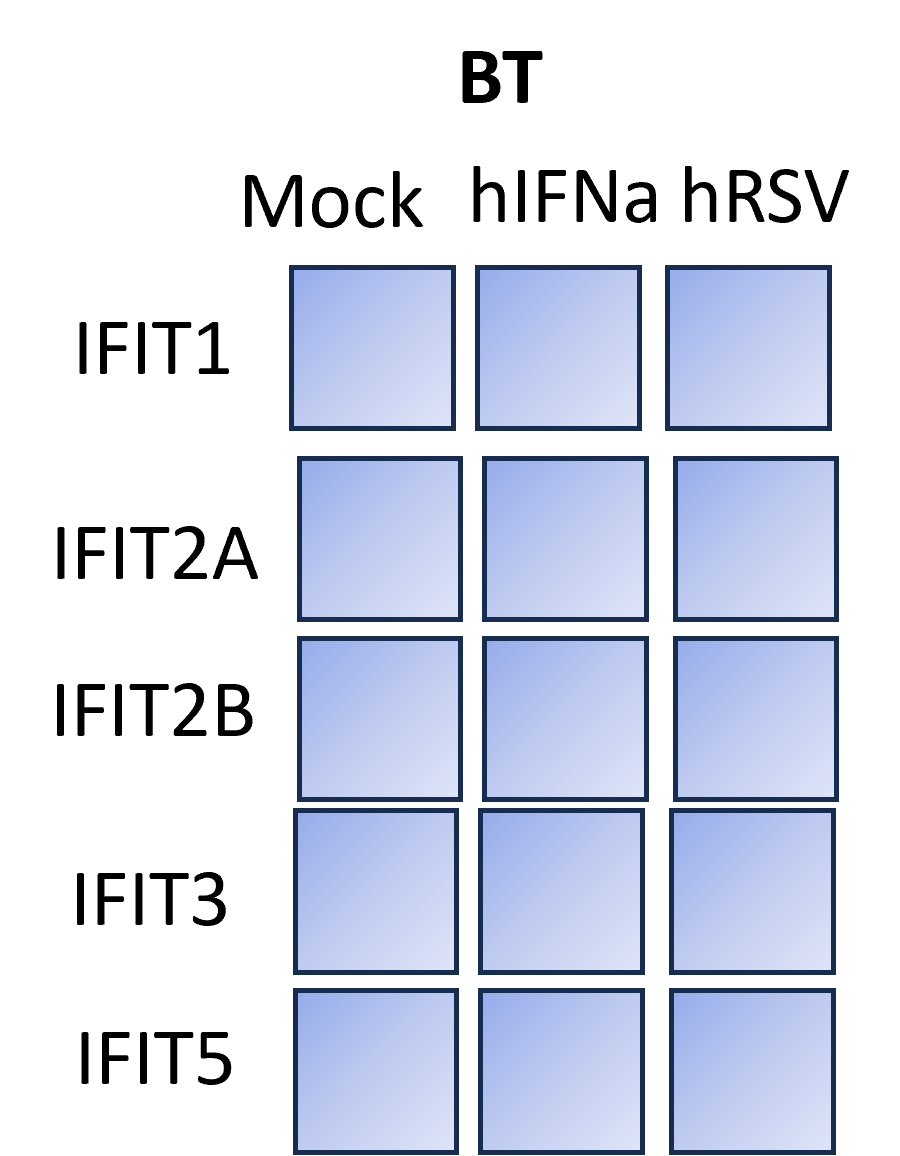
\includegraphics[width=1\linewidth]{07. Chapter 2/Figs/04. Localisation/03. bt merges.png}
    \caption[BT localisation mergers.]{BT localisation mergers.}
    \label{BTlocalisation mergers.}
\end{figure}


\begin{figure}
    \centering
    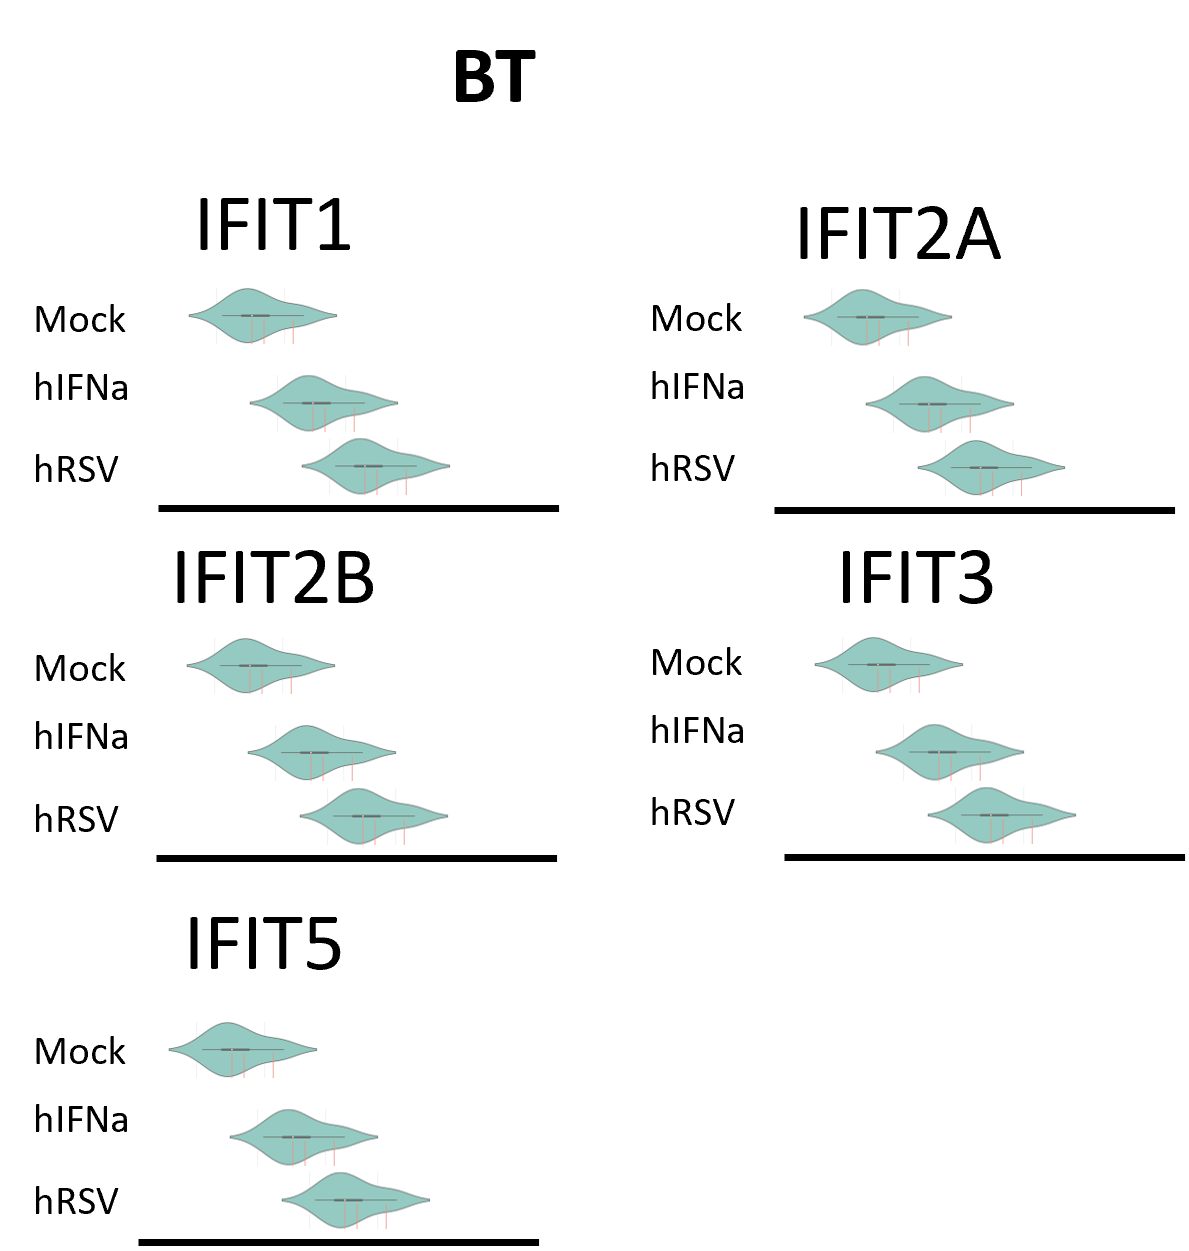
\includegraphics[width=1\linewidth]{07. Chapter 2/Figs/04. Localisation/04. bt plots.png}
    \caption[BT localisation plots.]{BT localisation plots.}
    \label{BT localisation plots.}
\end{figure}

\section{Discussion} \label{Discussion}
Recap human induction \newline
Recap human expression \newline
Recap human localisation




\nomenclature[IU]{IU}{International Units}
\nomenclature[PS]{PS}{Primer Set}